\documentclass[24pt]{beamer}
\usepackage[utf8]{inputenc}
\usepackage[utf8]{vietnam}
\usepackage{amsmath}
\usepackage{amsfonts}
\usepackage{amssymb}
\usepackage{graphicx}
\usepackage{multimedia}
\usepackage{tikz}
\usetikzlibrary{positioning}
\usetikzlibrary{arrows}
\usetikzlibrary{decorations.markings}
\usepackage{xcolor}
\usepackage{utopia} %font utopia imported
\usepackage{siunitx}
\usepackage[american,cuteinductors,smartlabels]{circuitikz}
\usepackage{ragged2e}
\usepackage{etoolbox}

\mode<beamer>{\usetheme{CambridgeUS}}

\usecolortheme{default}

\usepackage{hyperref}
\hypersetup{pdfpagemode=FullScreen} %mode FullScreen with beamer

\apptocmd{\frame}{}{\justifying}{} % Allow optional arguments after frame.

\usepackage{comment}

\makeatletter
\let\insertuniversity\relax
\newcommand\universitytitle{TRƯỜNG ĐH}

\let\insertclass\relax
\newcommand\classtitle{Lớp}

\let\insertcourse\relax
\newcommand\coursetitle{Môn học}

\mode<all>
{
  \newcommand\university[1]{\def\insertuniversity{#1}}
  
  \newcommand\class[1]{\def\insertclass{#1}}
  
  \newcommand\course[1]{\def\insertcourse{#1}}
  \titlegraphic{}
}

\defbeamertemplate*{title page}{supdefault}[1][]
{
  \begingroup
    \centering
    \ifx\insertuniversity\relax\relax\else
    \begin{beamercolorbox}[sep=2pt,center,#1]{author}
      \hspace{-.15cm}\scriptsize\universitytitle~\insertuniversity
    \end{beamercolorbox}\fi
    
    \begin{beamercolorbox}[sep=8pt,center,#1]{title}
      \usebeamerfont{title}\normalsize\inserttitle\par%
      \ifx\insertsubtitle\@empty\relax%
      \else%
        \vskip0.25em%
        {\usebeamerfont{subtitle}\usebeamercolor[fg]{subtitle}\insertsubtitle\par}%
      \fi%     
    \end{beamercolorbox}%
    \vskip.5em\par

    \vspace{-.4cm}
    \ifx\insertcourse\relax\relax\else
    \begin{beamercolorbox}[sep=6pt,center,#1]{author}
      \usebeamerfont{author}\footnotesize\coursetitle:~\insertcourse
    \end{beamercolorbox}\fi

    \vspace{-.3cm}
    \ifx\insertclass\relax\relax\else
    \begin{beamercolorbox}[sep=6pt,center,#1]{author}
      \usebeamerfont{author}\footnotesize\classtitle:~\insertclass
    \end{beamercolorbox}\fi

    \vspace{-.3cm}
    \begin{beamercolorbox}[sep=6pt,center,#1]{author}
      \usebeamerfont{author}\hspace{-.23cm}\footnotesize\insertauthor
    \end{beamercolorbox}
    %\begin{beamercolorbox}[sep=8pt,center,#1]{institute}
      %\usebeamerfont{institute}\insertinstitute
    %\end{beamercolorbox}
    \vspace{-.4cm}
    \begin{beamercolorbox}[sep=8pt,center,#1]{date}
      \usebeamerfont{date}\footnotesize\insertdate
    \end{beamercolorbox}\vskip0.5em
    {\usebeamercolor[fg]{titlegraphic}\inserttitlegraphic\par}
  \endgroup
  \vfill
}
\setbeamertemplate{title page}[supdefault][colsep=-4bp,rounded=true,shadow=\beamer@themerounded@shadow]\makeatother

%Title page
\title[Động cơ điện một chiều]{\emph{Chủ đề báo cáo}\\ Điều khiển tốc độ vòng hở ĐC DC từ nguồn AC 1 pha và 3 pha}
\author[Cơ sở Truyền động điện]{GVHD: Hồ Minh Nhị \and Nhóm SVTH: Nhóm 1}
\course{Cơ sở Truyền động điện}
\class{Công nghệ, kỹ thuật điện, điện tử}
\university{KỸ THUẬT -- CÔNG NGHỆ CẦN THƠ}
\date[Nhóm 1]{\today}

%\logo{
\includegraphics[height=1.3cm]{logo_ctut.pdf}}

\AtBeginSection[]
{
  \begin{frame}
    \frametitle{Nội dung báo cáo}
    \justifying
    \tableofcontents[currentsection]
  \end{frame}
}
\definecolor{doden}{RGB}{204, 0, 0}
\newcommand{\noibat}[1]{\textcolor{red}{#1}}
\newcommand{\noibatn}[1]{\textcolor{blue}{#1}}
\newcommand{\drawe}{\draw[line width=1.2pt]}
\newcommand{\pfm}[1]{\left({#1}\right)}
\newcommand{\viet}[2]{#1_{\text{\textit{#2}}}}
\begin{document}
%http://tex.stackexchange.com/questions/82794/removing-page-number-from-title-frame-without-changing-the-theme
\bgroup
\makeatletter
\setbeamertemplate{footline}
{
  \leavevmode%
  \hbox{%
  \begin{beamercolorbox}[wd=.333333\paperwidth,ht=2.25ex,dp=1ex,center]{author in head/foot}%
    \usebeamerfont{author in head/foot}\insertshortauthor\expandafter\beamer@ifempty\expandafter{\beamer@shortinstitute}{}{~~(\insertshortinstitute)}
  \end{beamercolorbox}%
  \begin{beamercolorbox}[wd=.333333\paperwidth,ht=2.25ex,dp=1ex,center]{title in head/foot}%
    \usebeamerfont{title in head/foot}\insertshorttitle
  \end{beamercolorbox}%
  \begin{beamercolorbox}[wd=.333333\paperwidth,ht=2.25ex,dp=1ex,right]{date in head/foot}%
    \usebeamerfont{date in head/foot}\insertshortdate{}\hspace*{2em}
%    \insertframenumber{} / \inserttotalframenumber\hspace*{2ex} 
    \hspace*{6ex}
  \end{beamercolorbox}}%
  \vskip0pt%
}

\begin{frame}
\titlepage
\end{frame}
\egroup

\setcounter{framenumber}{0}

%--------------------------------------------------------------------------------
%--------------------------------------------------------------------------------
% Danh sách thành viên
\begin{frame}{Danh sách thành viên}
%	\vspace{-1cm}
	\begin{footnotesize}
	\begin{columns}
		\column{0.6\textwidth}
		\begin{enumerate}
			\item Nguyễn Văn Bảy
			\item Nguyễn Văn Đình
			\item Nguyễn Hoàng Hận
			\item Thi Minh Nhựt
			\item Phạm Thanh Quý
			\item Hồ Minh Thành
			\end{enumerate}

		\column{.6\textwidth}
		\begin{enumerate}	% Danh sach tiep theo
			\setcounter{enumi}{6}
			\item Nguyễn Văn Tiến
			\item Liên Thái Trường
			\item Trần Thanh Tú
			\item Bùi Trọng Tuấn
			\item Lư Anh Tuấn
			\item Nguyễn Bá Vọng
		\end{enumerate}
	\end{columns}
	\end{footnotesize}
\end{frame}

%--------------------------------------------------------------------------------
%--------------------------------------------------------------------------------
% Nội dung báo cáo
\begin	{frame}	%Trang muc luc
	\frametitle{Nội dung báo cáo}
	\tableofcontents
\end{frame}

%--------------------------------------------------------------------------------
%--------------------------------------------------------------------------------
% Điều khiển tốc độ từ bộ chỉnh lưu một pha
\section[Bộ chỉnh lưu một pha]{ĐK tốc độ động cơ DC từ bộ chỉnh lưu một pha}
\begin{frame}{ĐK tốc độ ĐC DC từ bộ chỉnh lưu một pha}
	\justifying
	\begin{block}{Chỉnh lưu một pha có điều khiển}
		\begin{itemize}
			\item Chỉnh lưu bán kỳ.
			\item Chỉnh lưu toàn kỳ.
		\end{itemize}
	\end{block}
\end{frame}
%--------------------------------------------------------------------------------
% Chỉnh lưu một pha bán kỳ có điều khiển
\subsection*{Chỉnh lưu bán kỳ}
\begin{frame}{Chỉnh lưu bán kỳ có ĐK}
	\begin{center}
		\vspace{-1cm}
		\justifying
		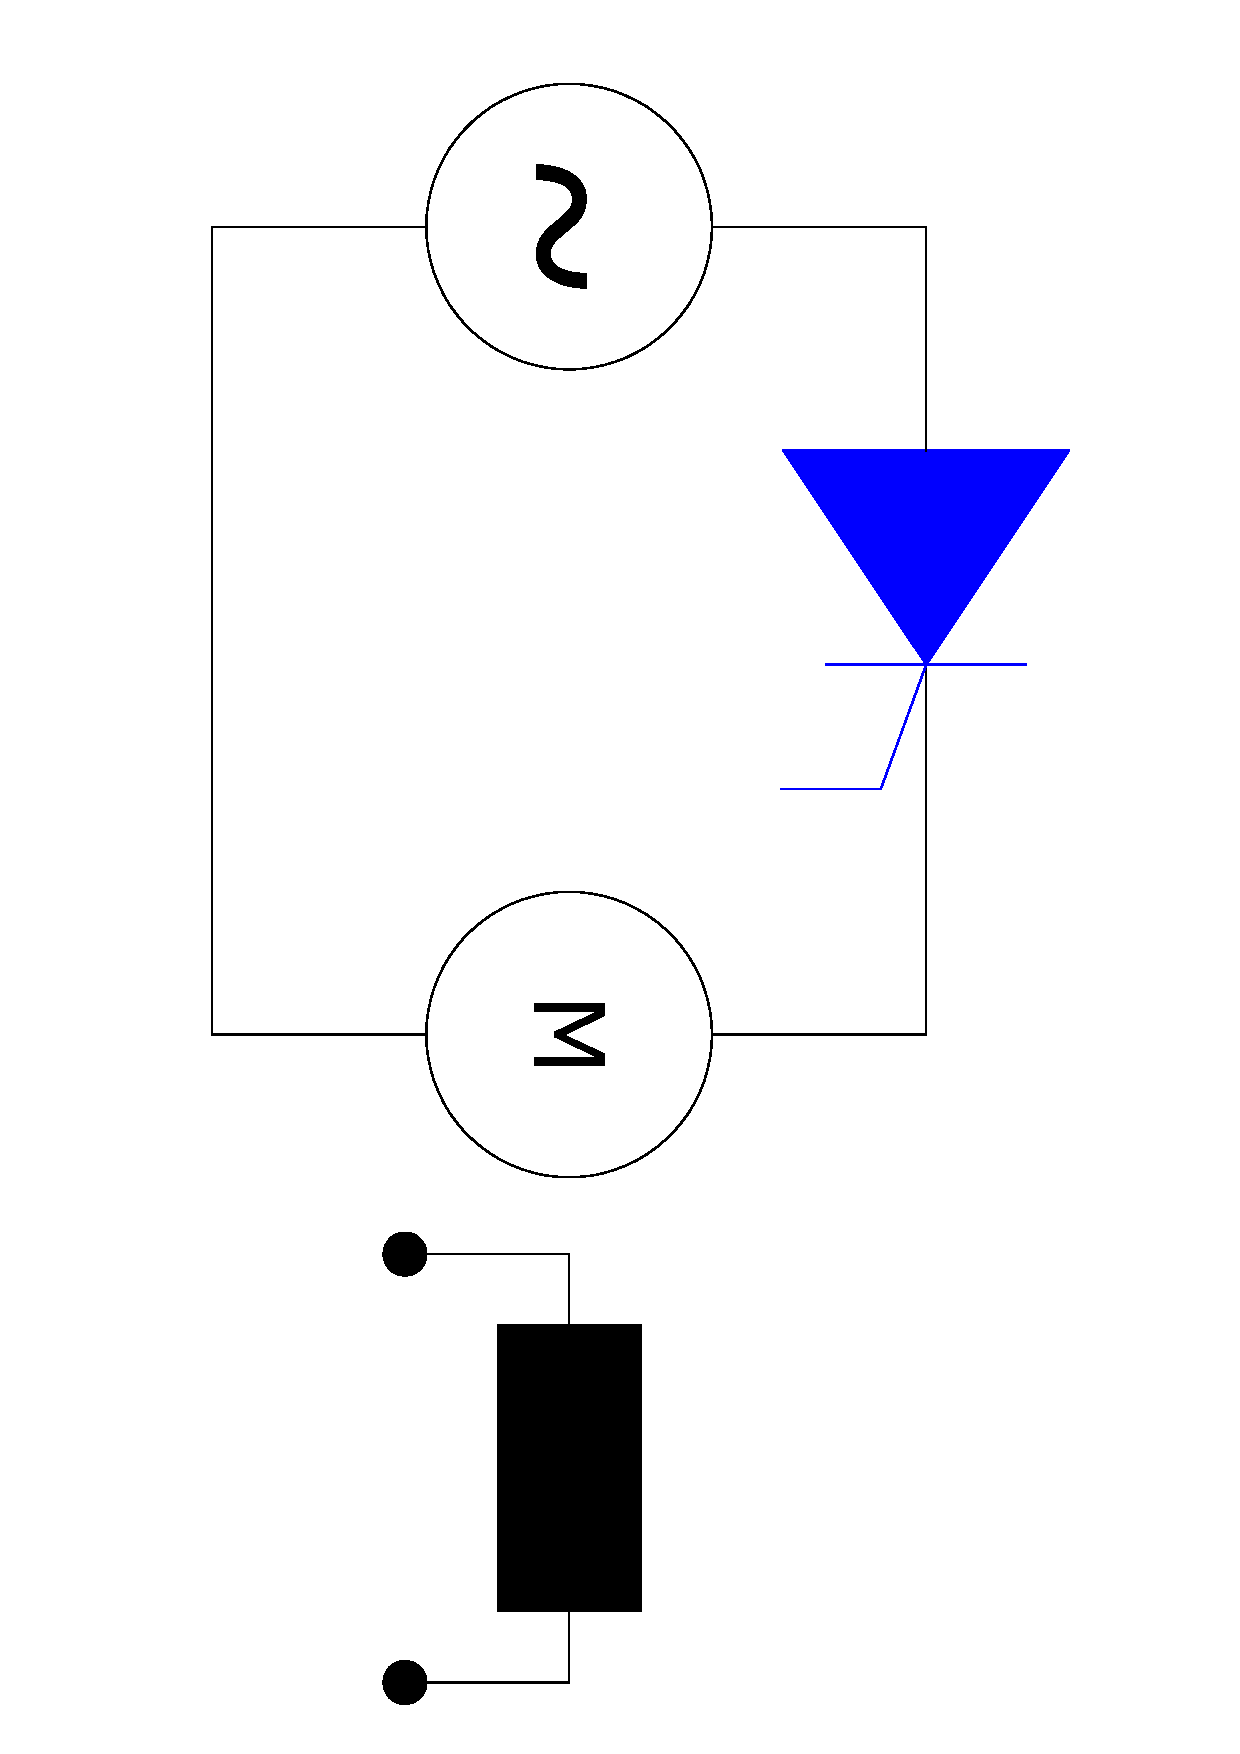
\includegraphics[scale=.35, angle=90]{images-chude6/chinh-luu-1pha-co-dieu-khien-tai-motor-DC.pdf} 
	\end{center}
\end{frame}

\begin{frame}{Chỉnh lưu bán kỳ có ĐK}
	\begin{center}
		\vspace{-.7cm}
		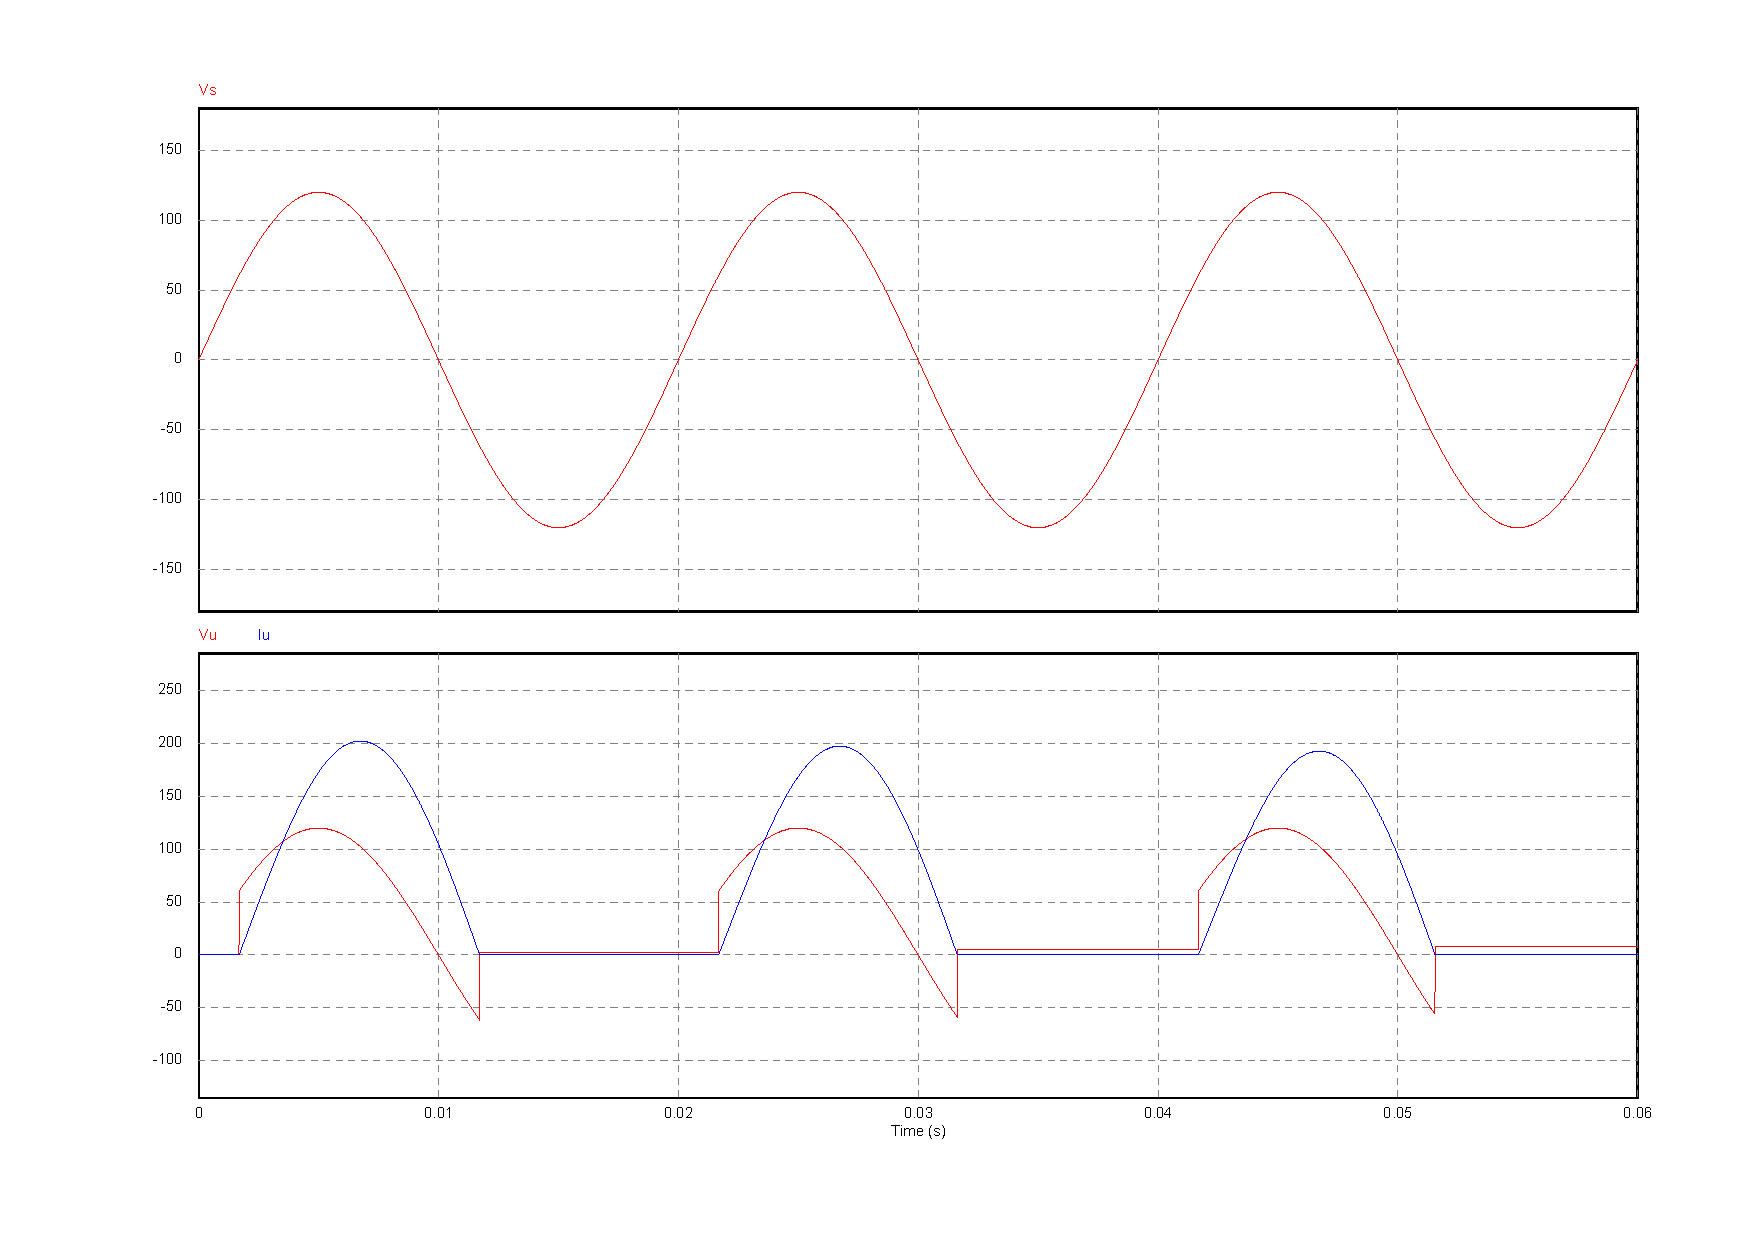
\includegraphics[scale=.35]{images-chude6/chinh-luu-1pha-co-dieu-khien-tai-motor-DC-plot-Vs-Vu-Iu-alpha-30.pdf} 
	\end{center}
\end{frame}

\begin{frame}{Chỉnh lưu bán kỳ có ĐK}
	\begin{block}{Nhận xét}
		Dòng cấp qua tải gián đoạn, độ nhấp nhô khá lớn, cho hiệu suất thấp, nên cấp cho động cơ có công suất nhỏ.
	\end{block}
\end{frame}

\begin{frame}{Chỉnh lưu bán kỳ có ĐK}
	\begin{picture}(100,100)
%	\vspace{-1.5cm}
		\put(0,-50){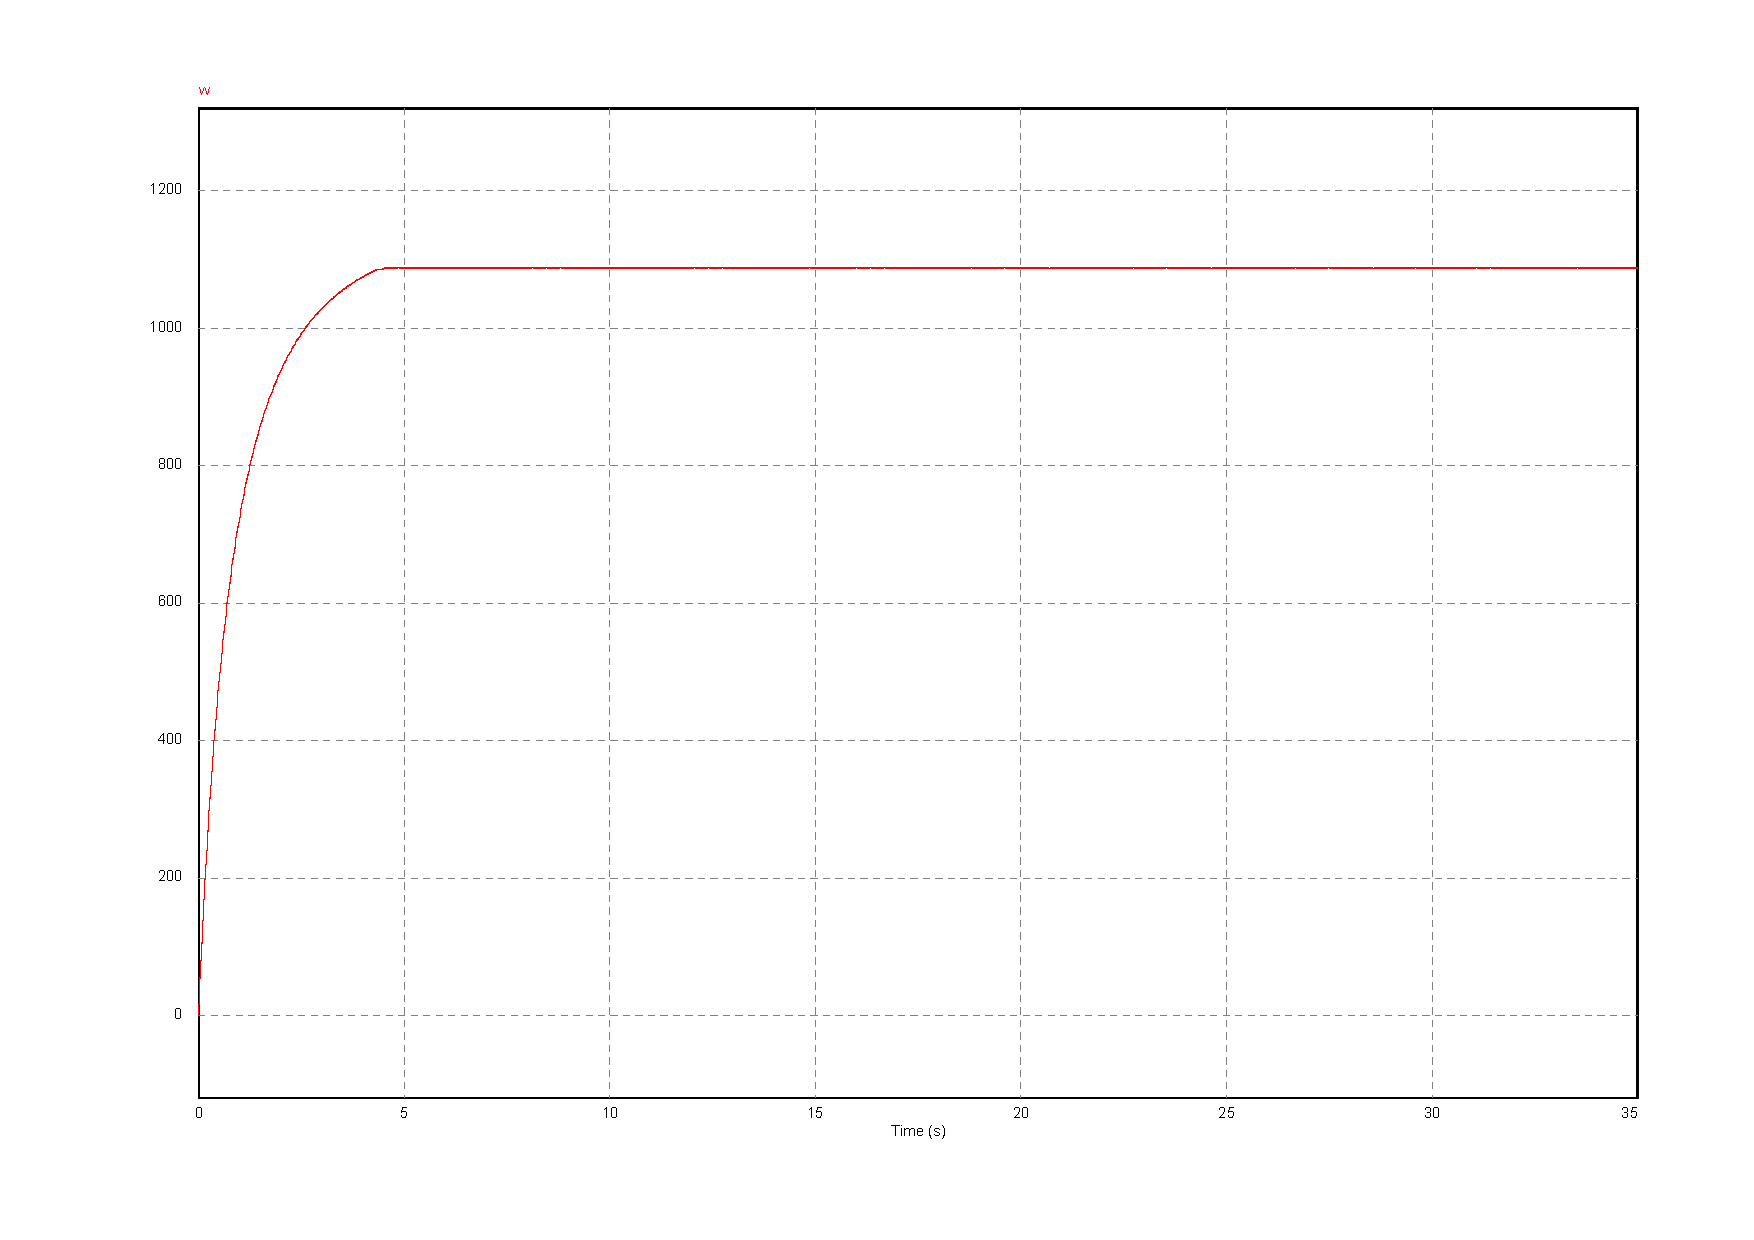
\includegraphics[scale=.33]{images-chude6/chinh-luu-1pha-co-dieu-khien-tai-motor-DC-plot-w-alpha-30.pdf}}
		\put(80,6){$\alpha = 30^0$}
	\end{picture}
\end{frame}

\begin{frame}{Chỉnh lưu bán kỳ có ĐK}
	\begin{picture}(100,100)
%	\vspace{-1.5cm}
		\put(0,-50){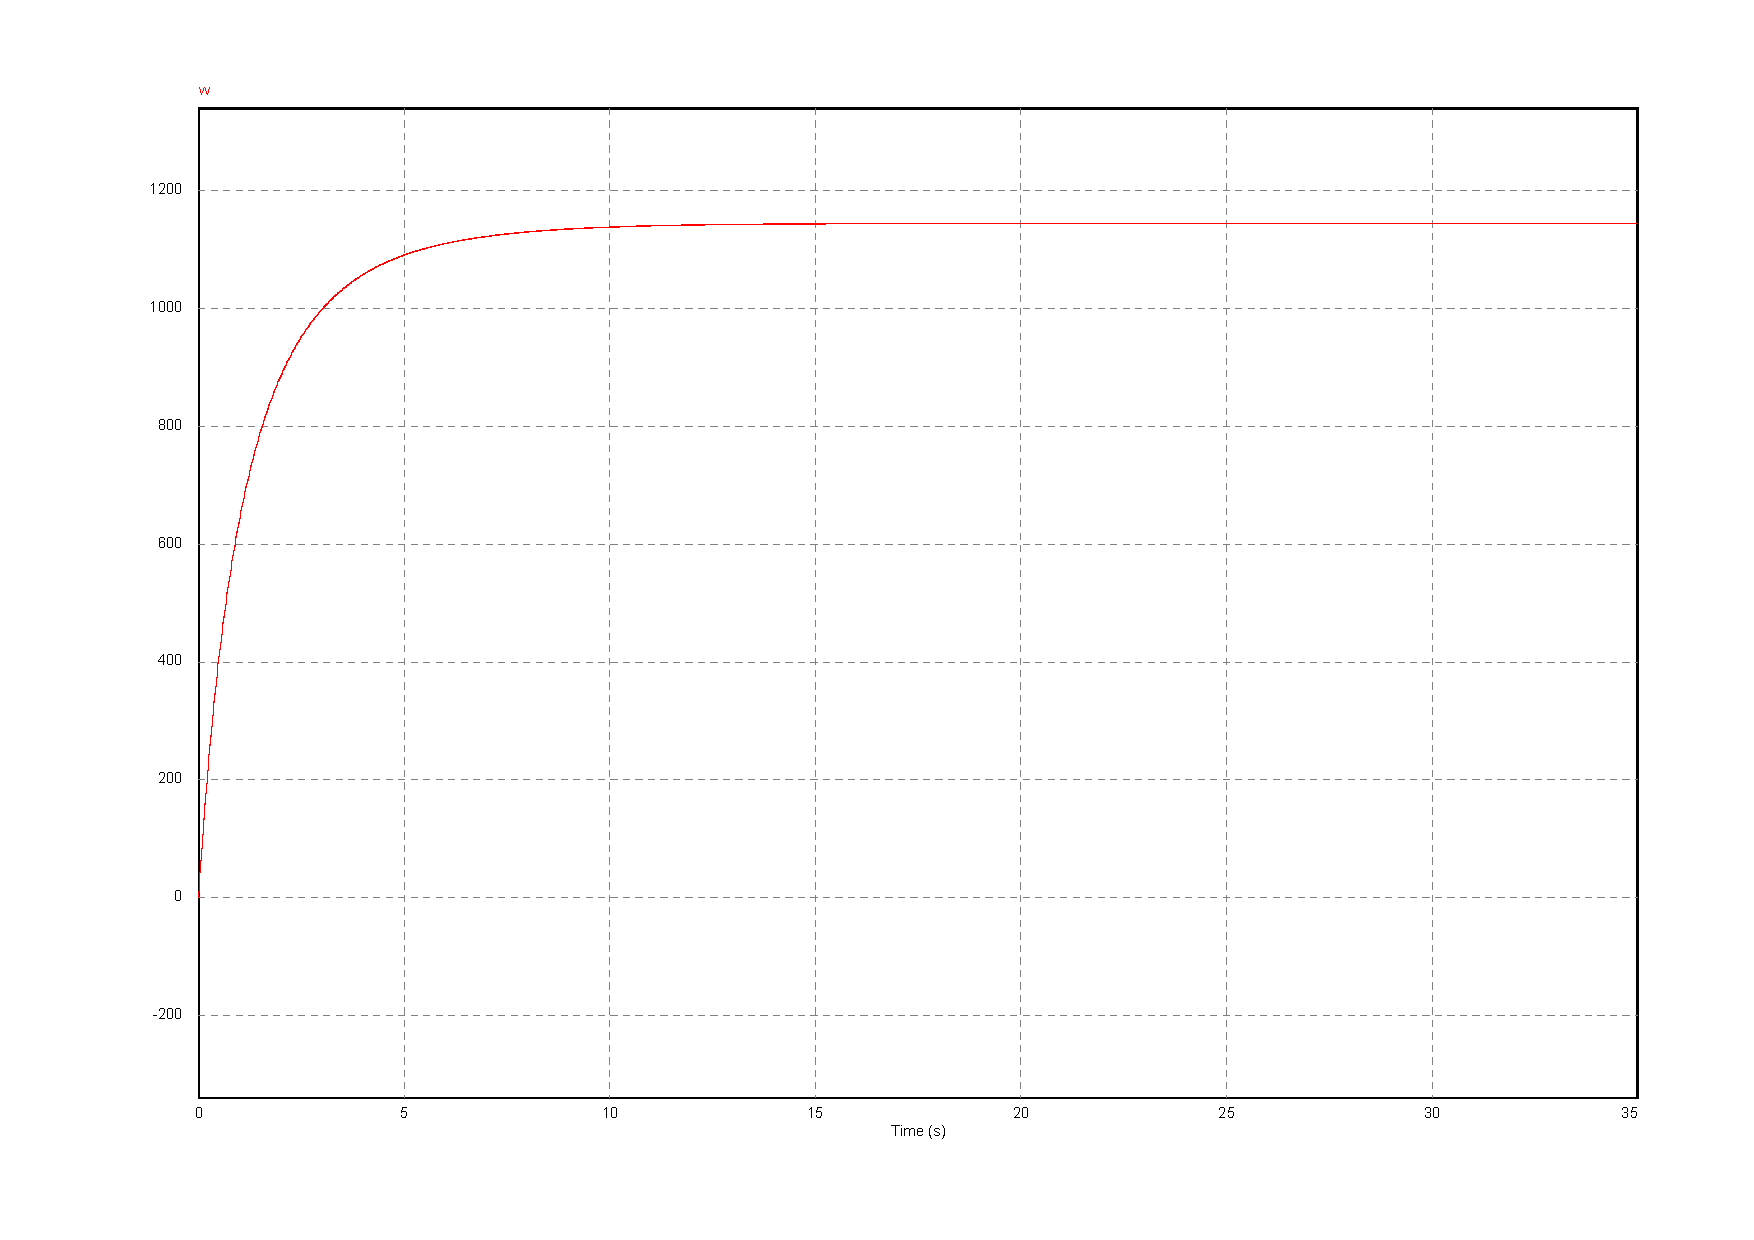
\includegraphics[scale=.33]{images-chude6/chinh-luu-1pha-co-dieu-khien-tai-motor-DC-plot-w-alpha-60.pdf}}
		\put(80,6){$\alpha = 60^0$}
	\end{picture}
\end{frame}

\begin{frame}{Chỉnh lưu bán kỳ có ĐK}
	\begin{picture}(100,100)
%	\vspace{-1.5cm}
		\put(0,-50){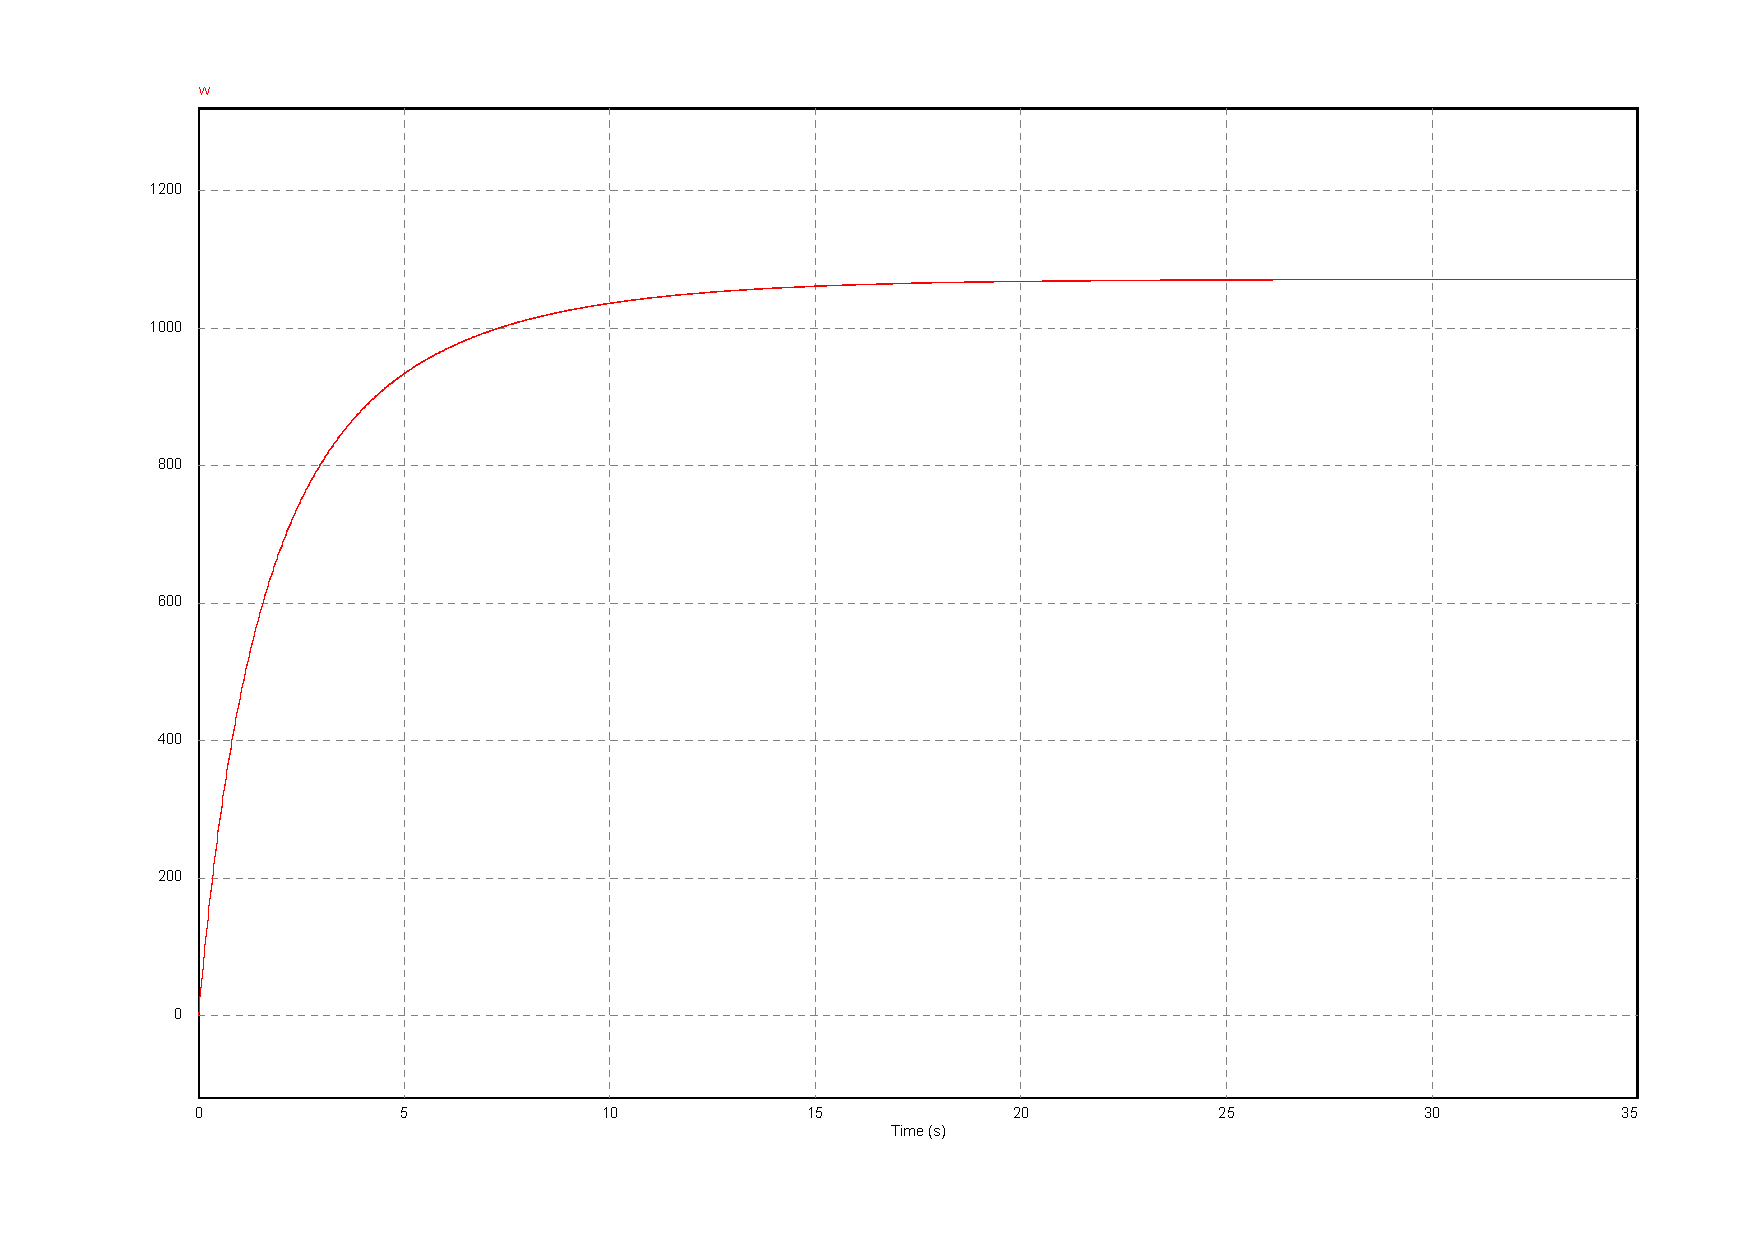
\includegraphics[scale=.33]{images-chude6/chinh-luu-1pha-co-dieu-khien-tai-motor-DC-plot-w-alpha-90.pdf}}
		\put(80,6){$\alpha = 90^0$}
	\end{picture}
\end{frame}

\begin{frame}{Chỉnh lưu bán kỳ có ĐK}
	\begin{picture}(100,100)
%	\vspace{-1.5cm}
		\put(0,-50){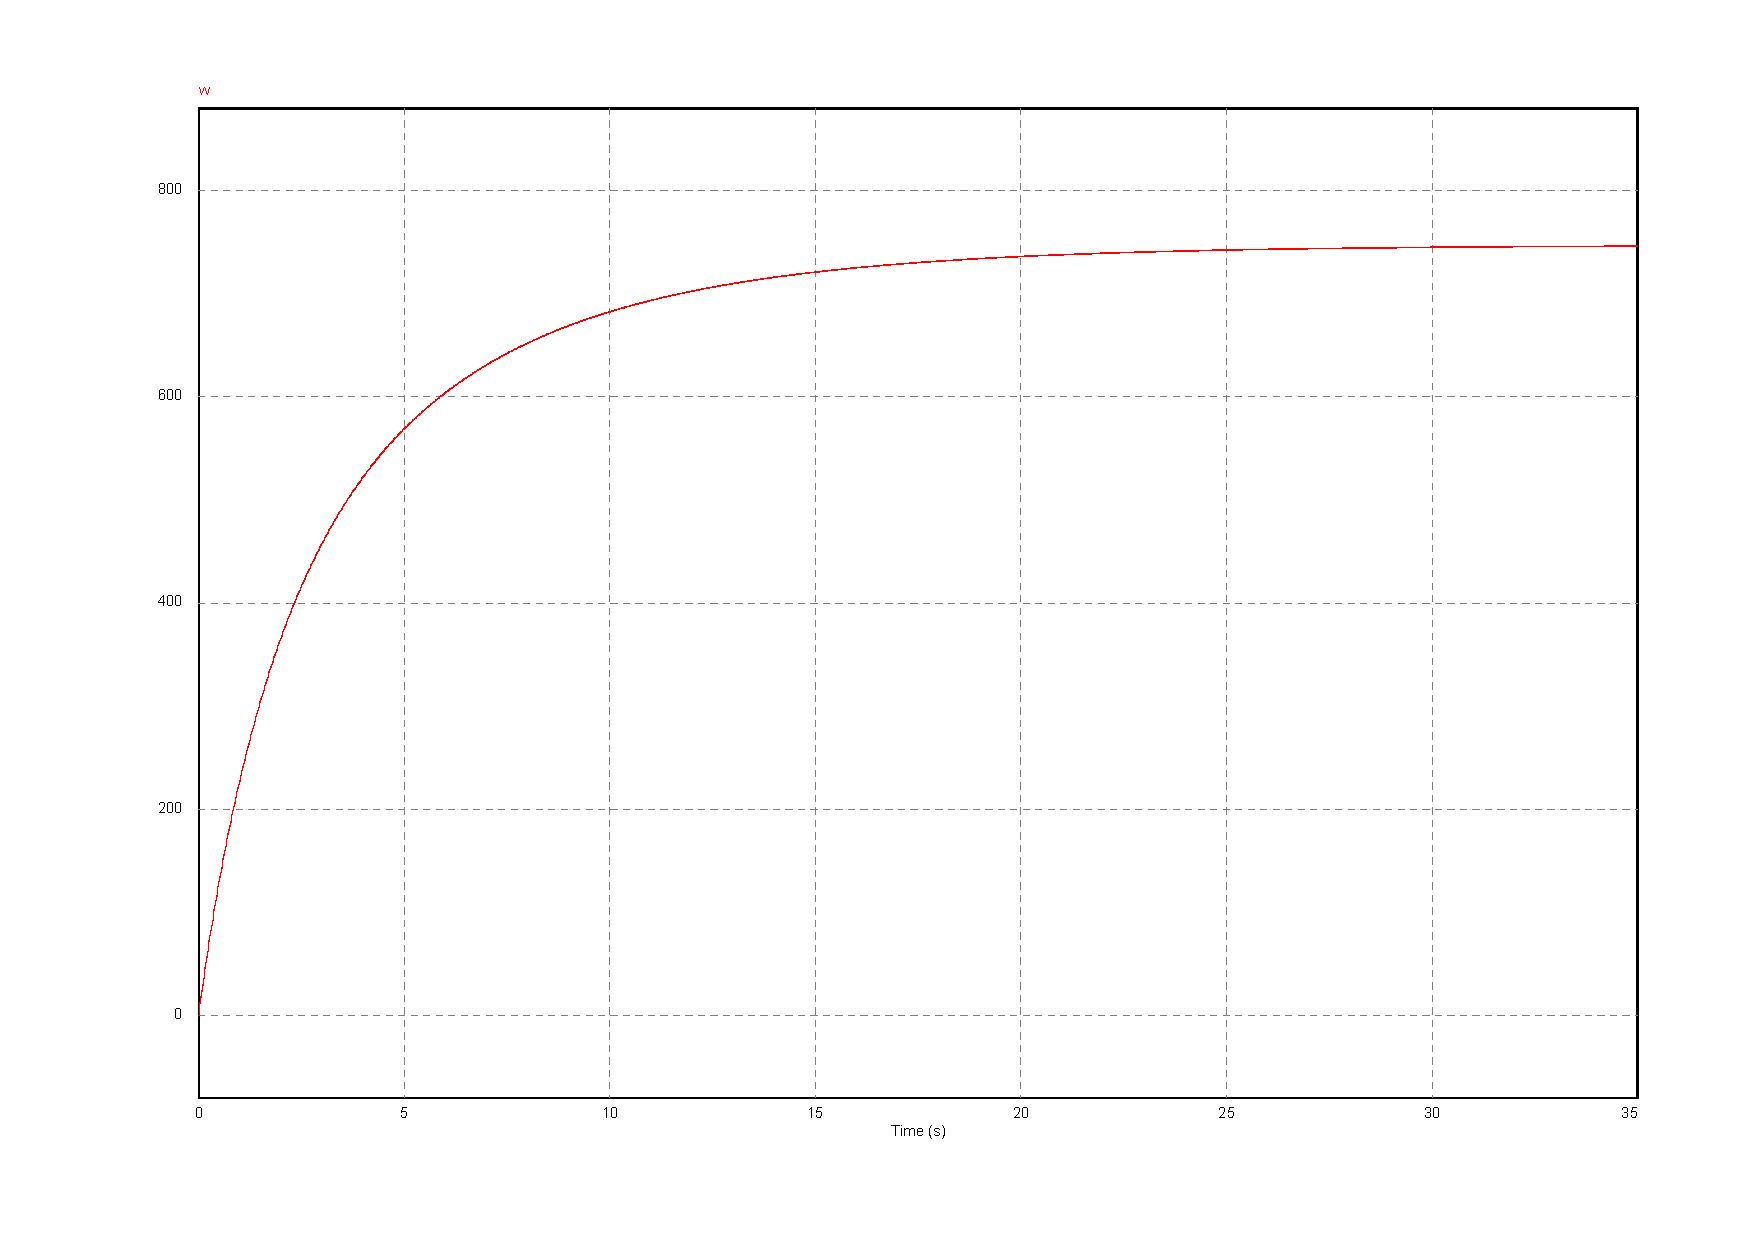
\includegraphics[scale=.33]{images-chude6/chinh-luu-1pha-co-dieu-khien-tai-motor-DC-plot-w-alpha-120.pdf}}
		\put(80,6){$\alpha = 120^0$}
	\end{picture}
\end{frame}

\begin{frame}{Chỉnh lưu bán kỳ có ĐK}
	\begin{center}
		\vspace{-2.5cm}
		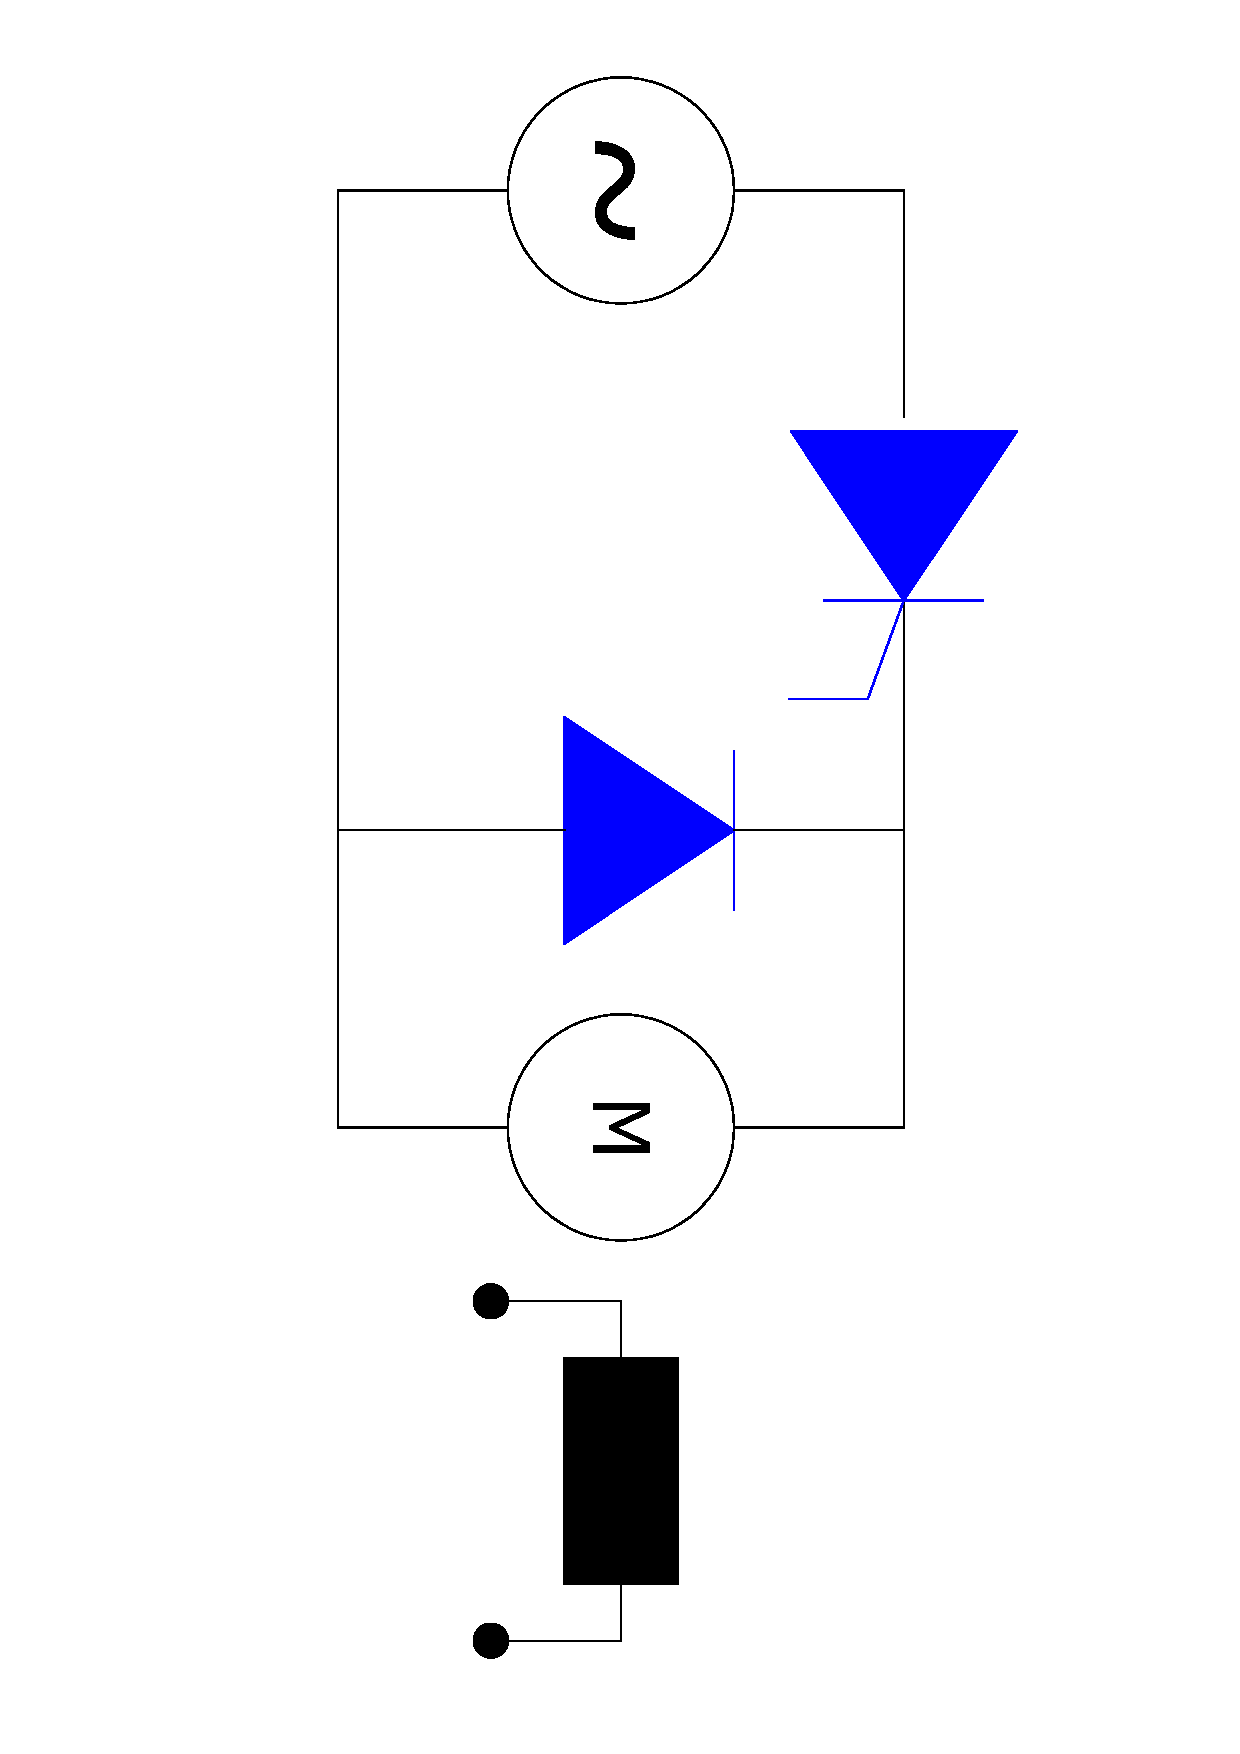
\includegraphics[scale=.4, angle=90]{images-chude6/chinh-luu-1pha-co-dieu-khien-them-diode-zero-tai-motor-DC.pdf} 
	\end{center}
\end{frame}

\begin{frame}{Chỉnh lưu bán kỳ có ĐK}
	\begin{center}
		\vspace{-.7cm}
		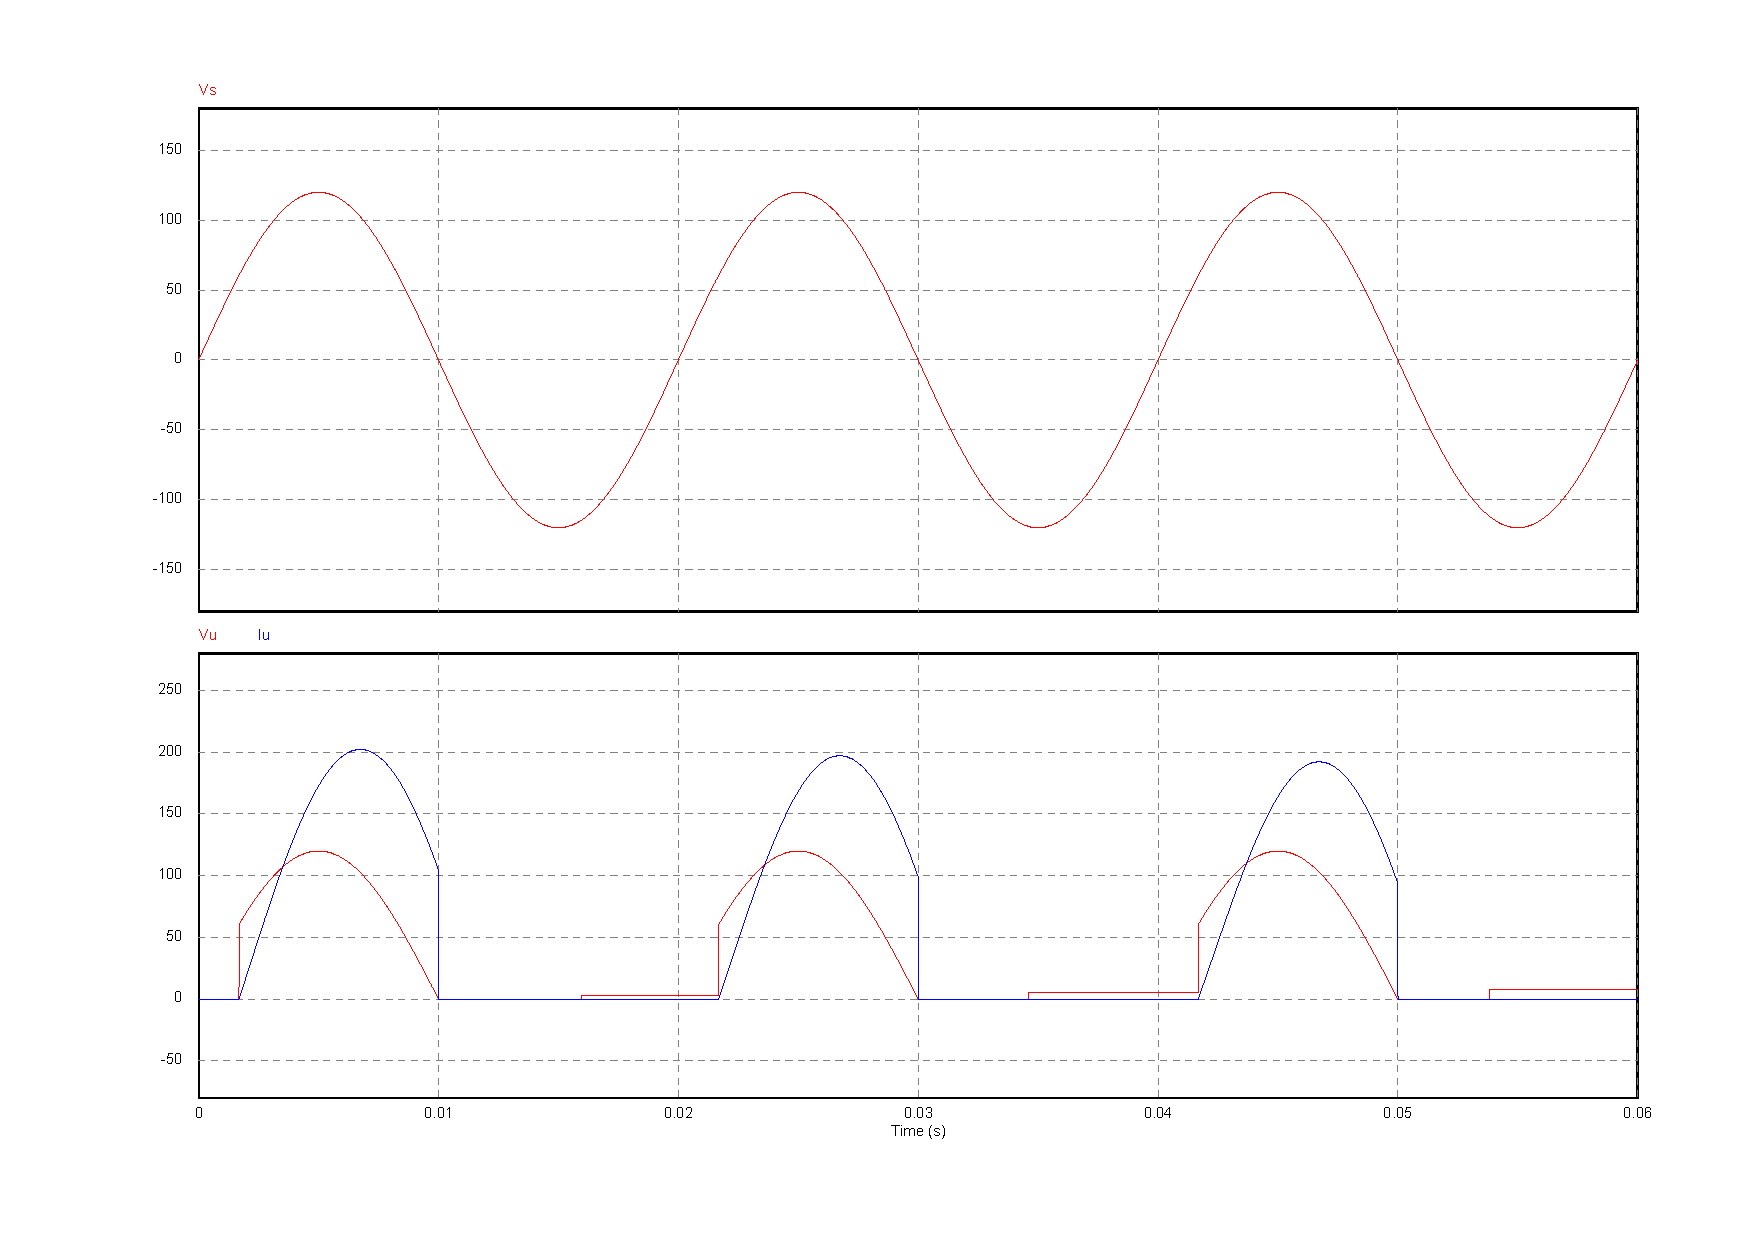
\includegraphics[scale=.35]{images-chude6/chinh-luu-1pha-co-dieu-khien-them-diode-zero-tai-motor-DC-plot-Vs-Vu-Iu-alpha-30.pdf} 
	\end{center}
\end{frame}

\begin{frame}{Chỉnh lưu bán kỳ có ĐK}
	\begin{center}
		\vspace{-.7cm}
		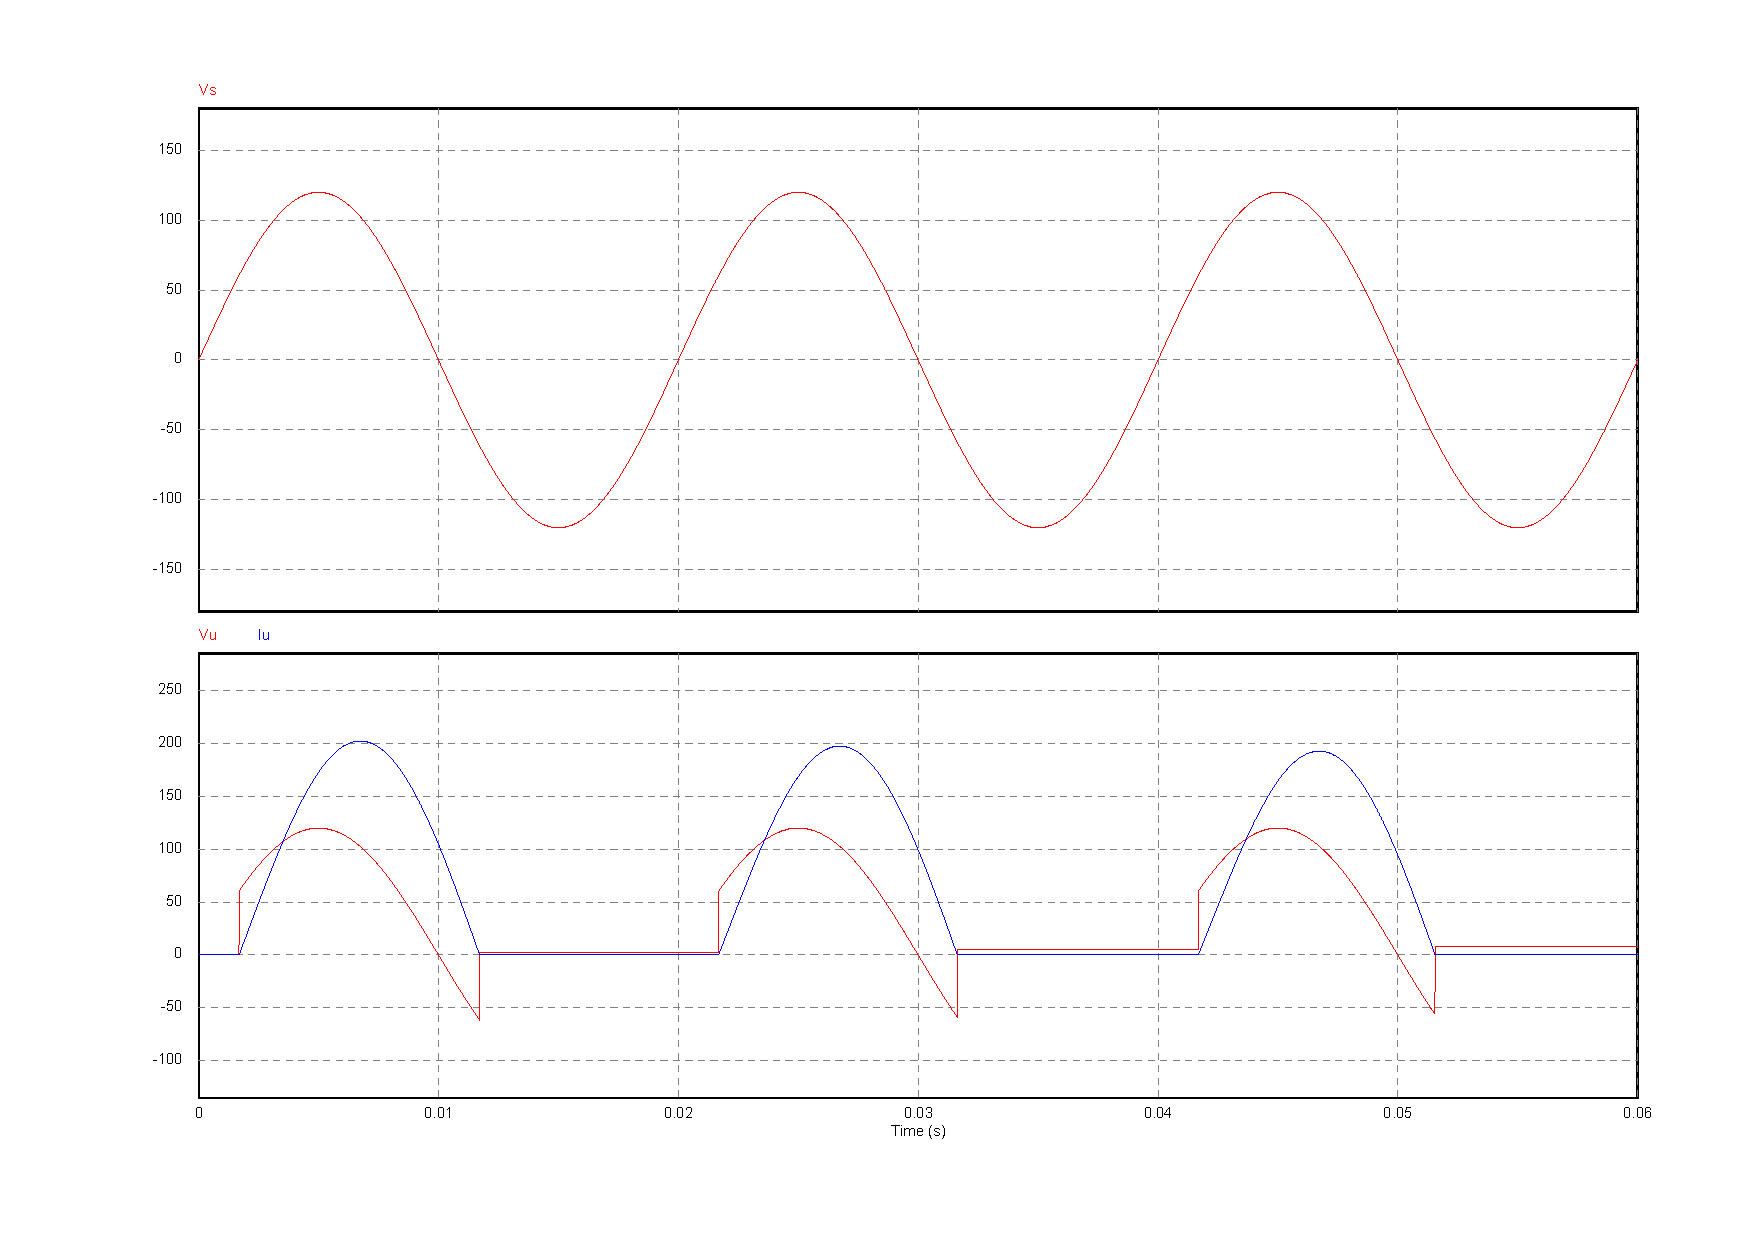
\includegraphics[scale=.2]{images-chude6/chinh-luu-1pha-co-dieu-khien-tai-motor-DC-plot-Vs-Vu-Iu-alpha-30.pdf}
		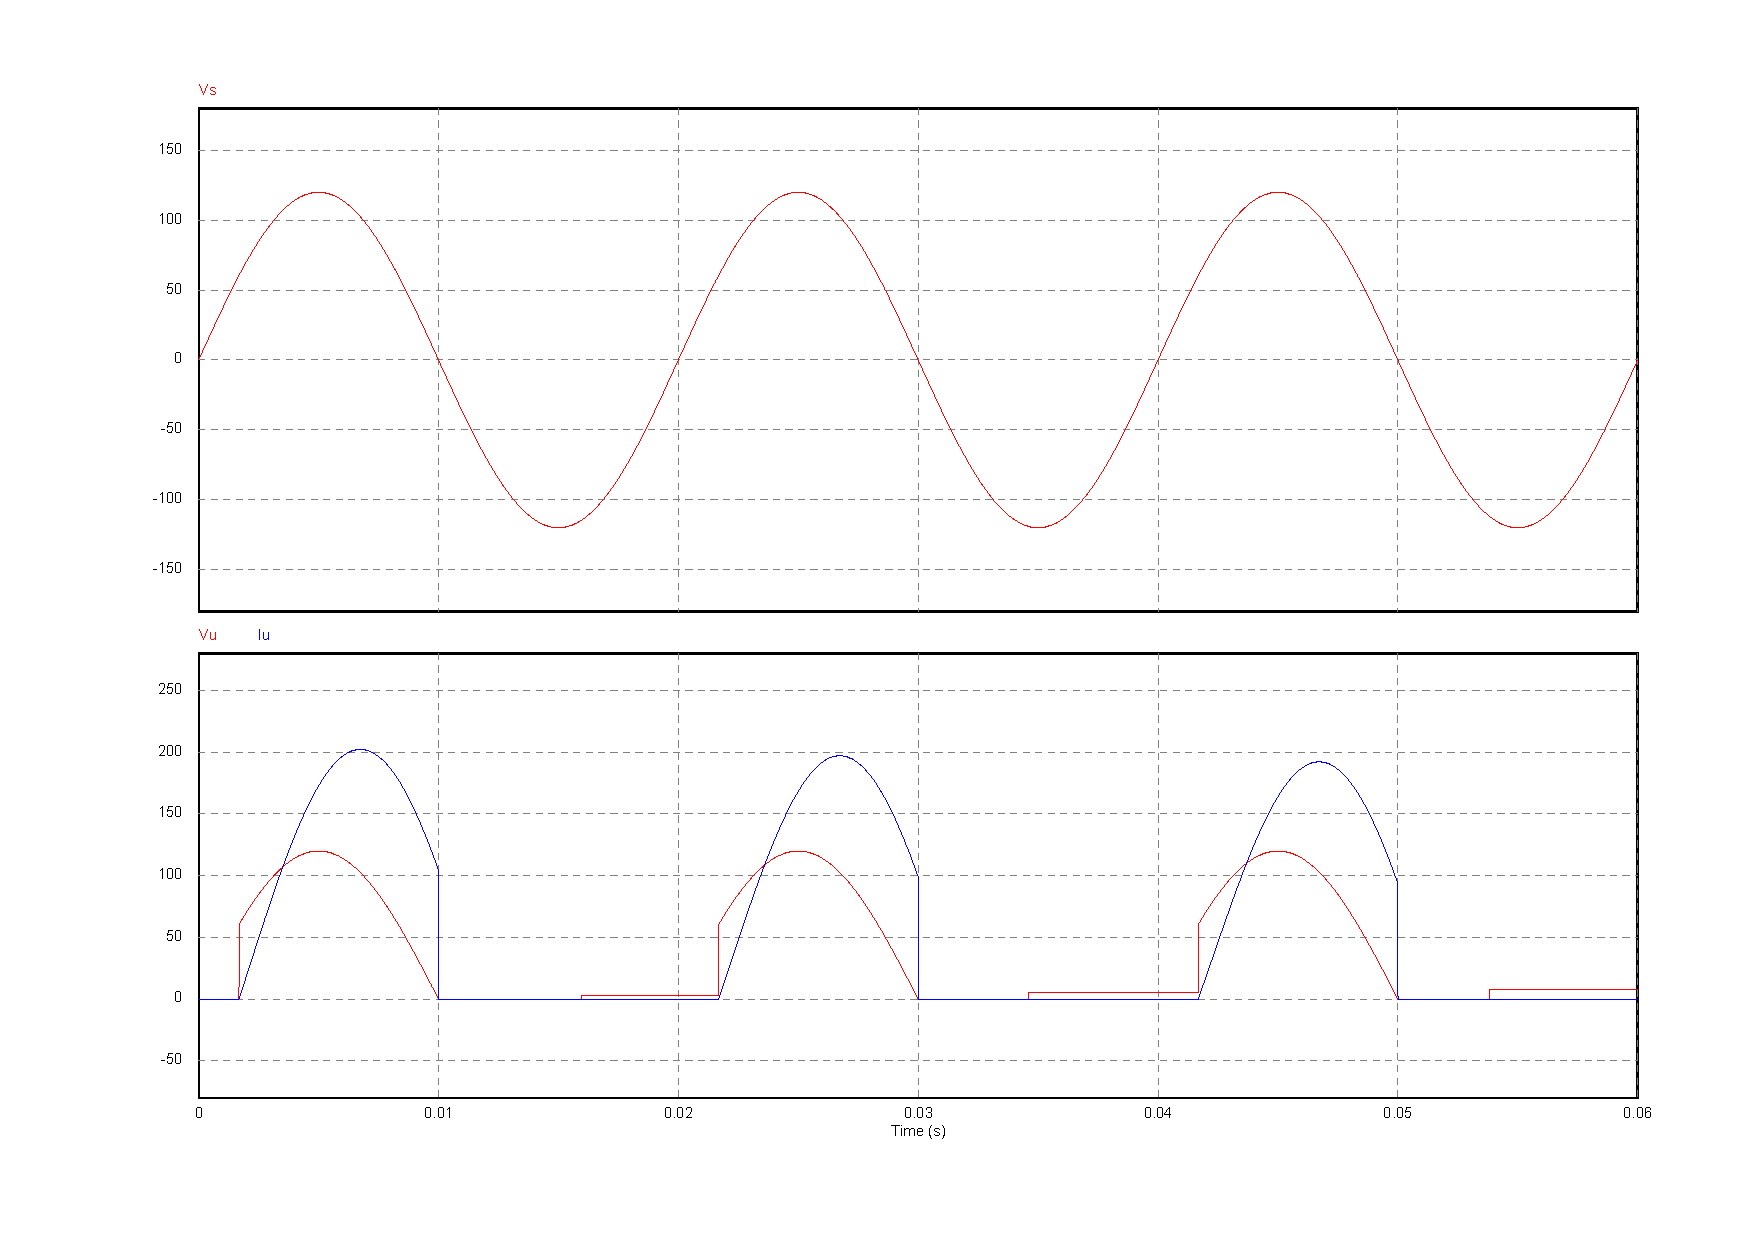
\includegraphics[scale=.2]{images-chude6/chinh-luu-1pha-co-dieu-khien-them-diode-zero-tai-motor-DC-plot-Vs-Vu-Iu-alpha-30.pdf} 
	\end{center}
\end{frame}

\begin{frame}{Chỉnh lưu bán kỳ có ĐK}
	\begin{block}{Nhận xét}
		\justifying
		Khi \alert{tăng góc kích $\alpha$} thì \alert{thời gian tăng tốc} của động cơ đến khi đạt tốc độ xác lập cũng \alert{tăng theo}.
	\end{block}
\end{frame}
%--------------------------------------------------------------------------------
% Chỉnh lưu toàn kỳ bán điều khiển
\begin{frame}{CLưu toàn kỳ bán ĐK}
	\begin{center}
		\vspace{-.7cm}
		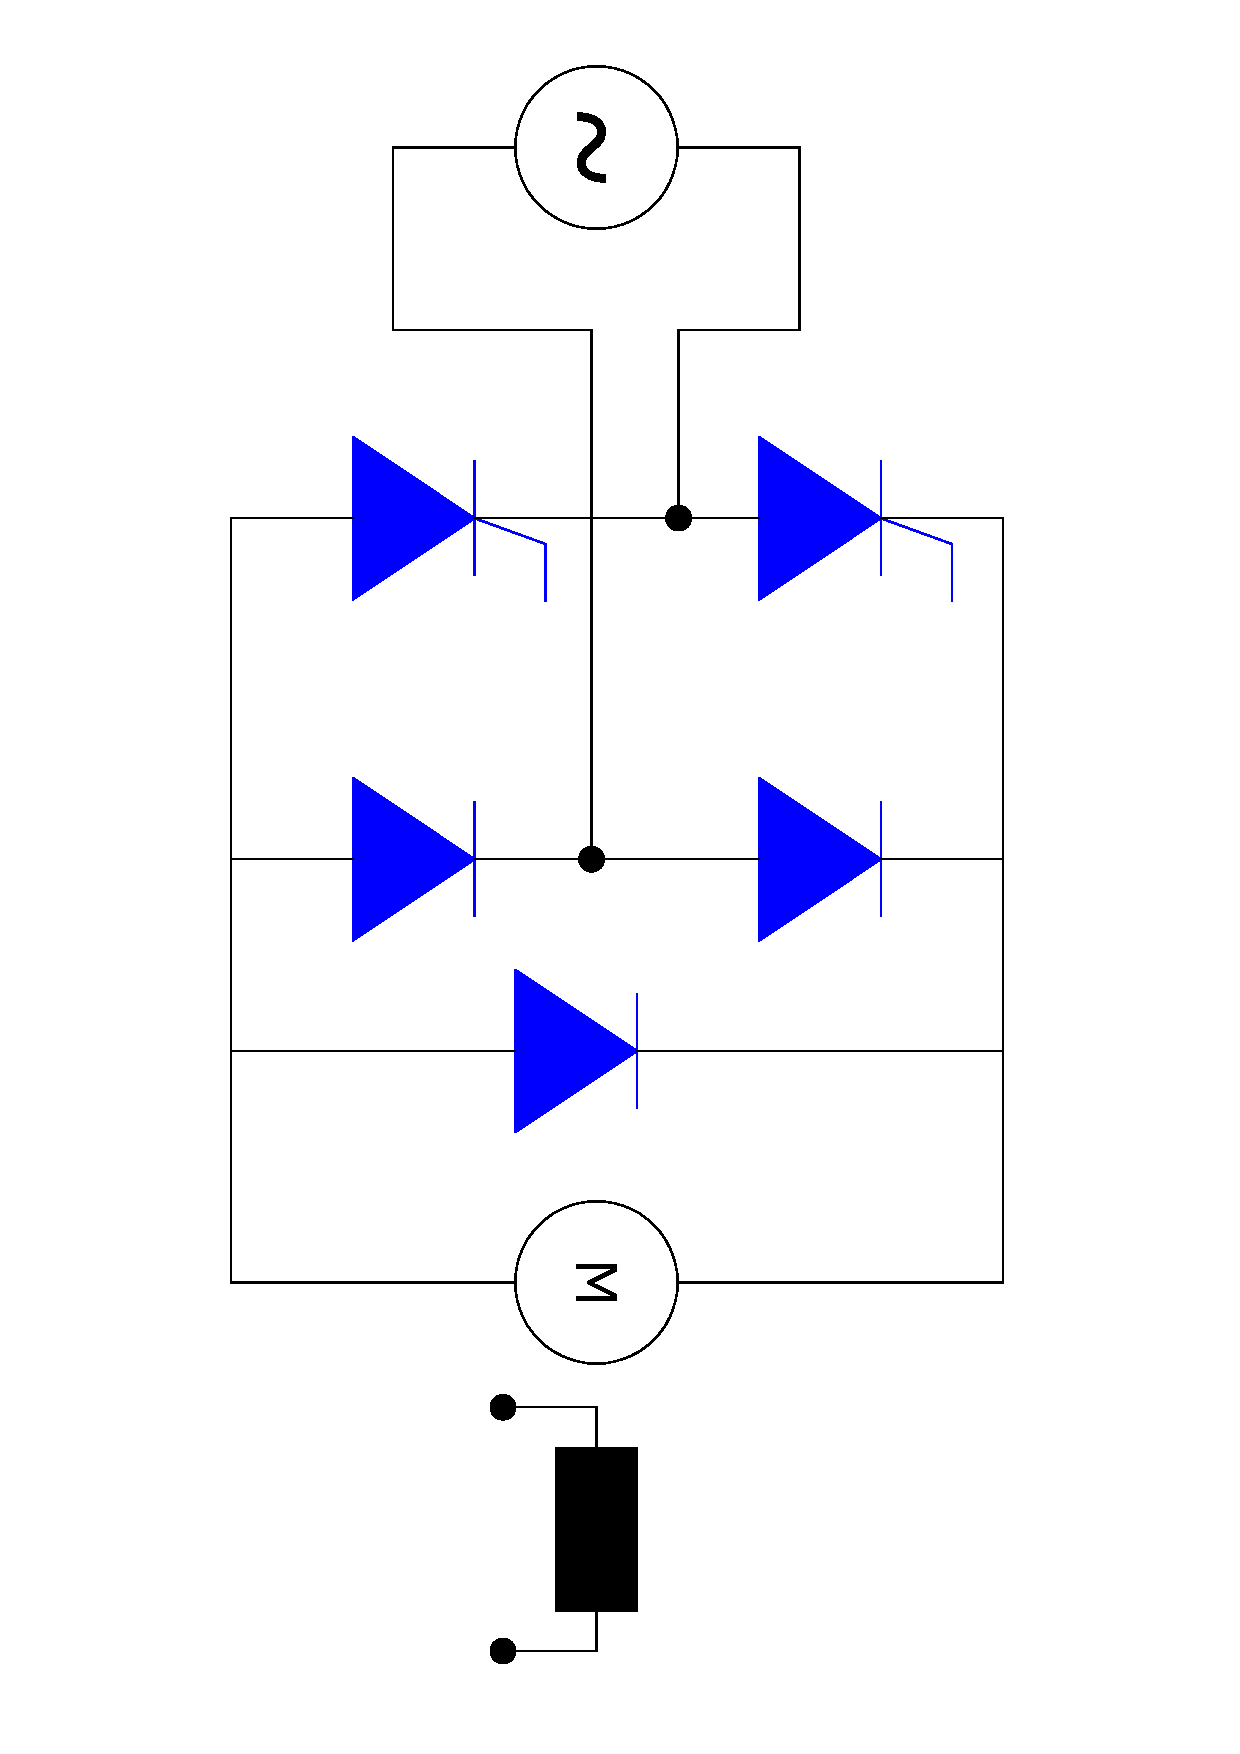
\includegraphics[scale=.35, angle=90]{images-chude6/chinh-luu-cau-1pha-ban-dieu-khien-bat-doi-xung-tai-motor-DC.pdf} 
	\end{center}
\end{frame}

\begin{frame}{CLưu toàn kỳ bán ĐK}
	\begin{center}
		\vspace{-.7cm}
		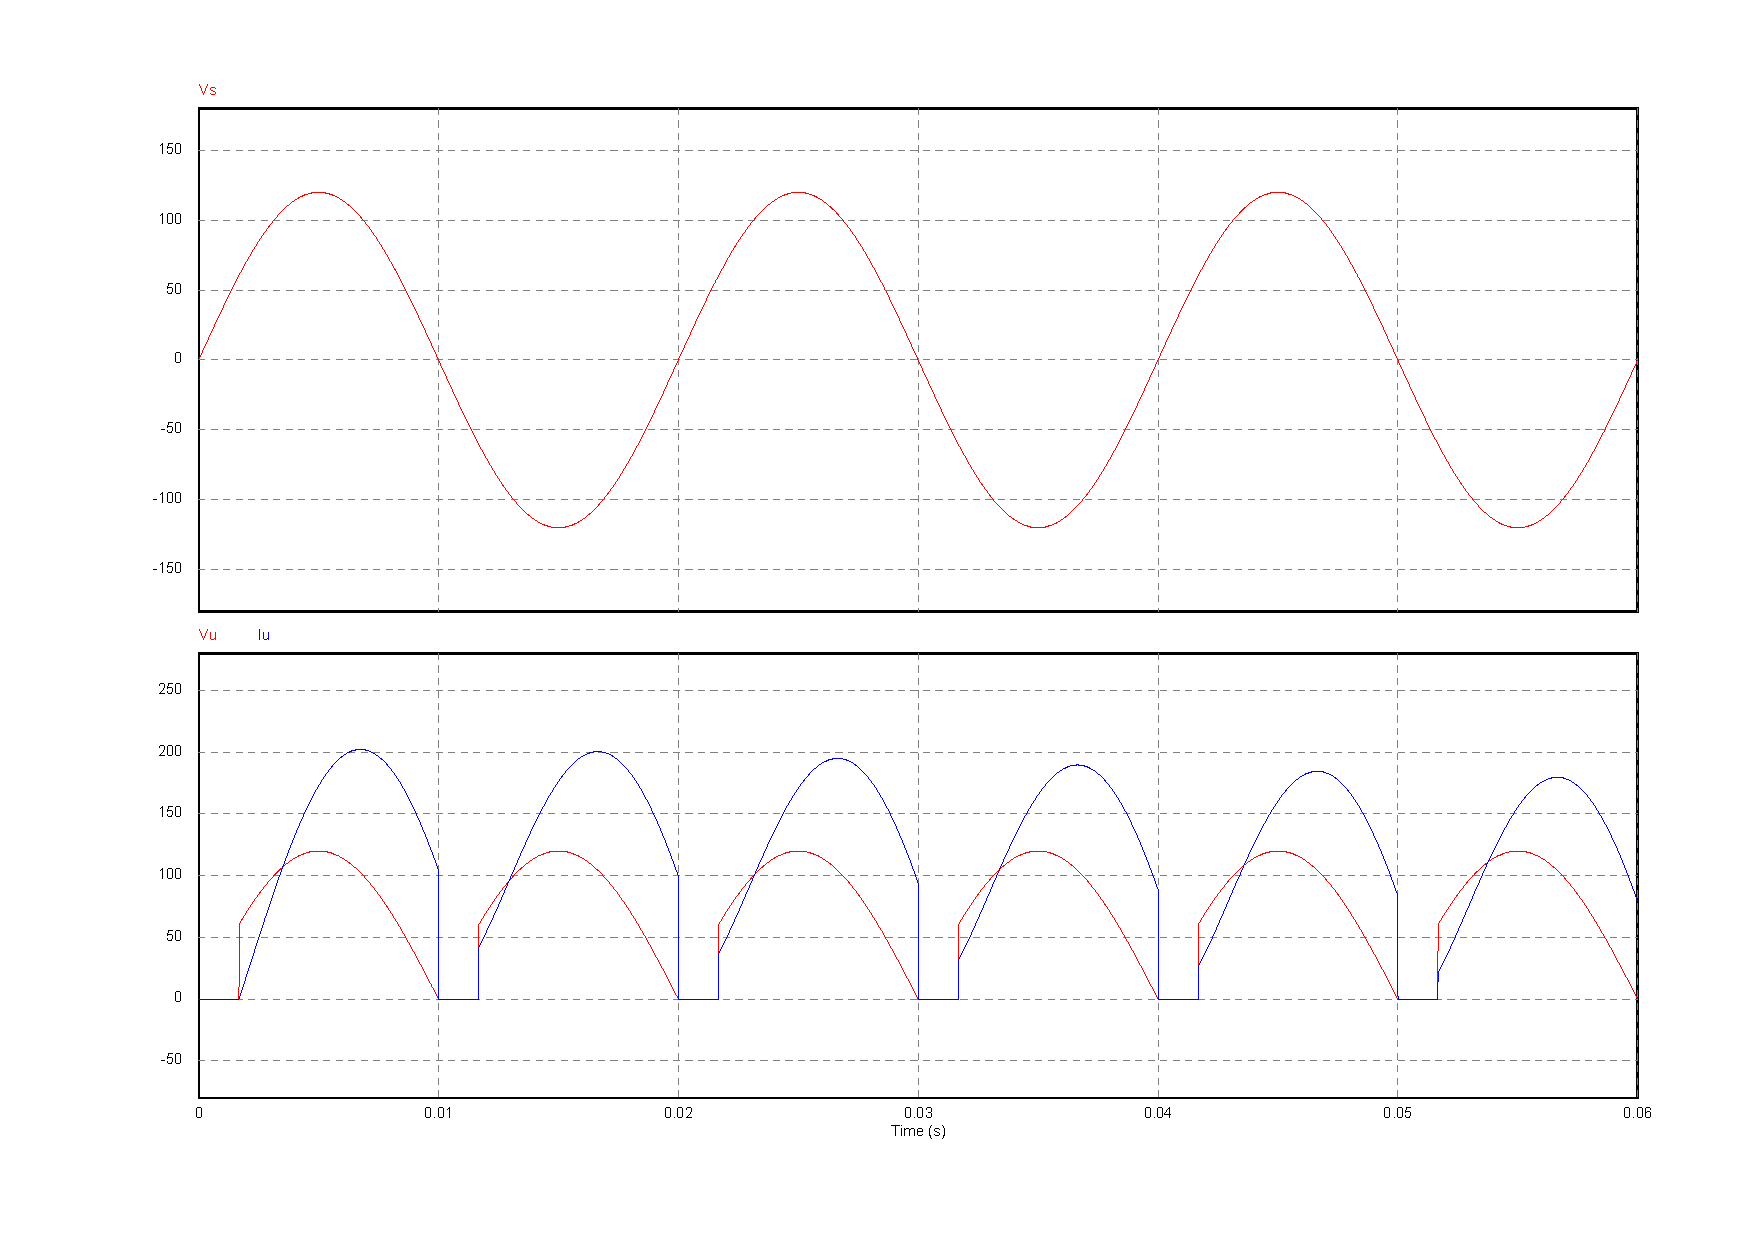
\includegraphics[scale=.35]{images-chude6/chinh-luu-cau-1pha-ban-dieu-khien-bat-doi-xung-tai-motor-DC-plot-Vs-Vu-Iu-alpha-30.pdf} 
	\end{center}
\end{frame}

\begin{frame}{CLưu toàn kỳ bán ĐK}
\begin{picture}(100,100)
%	\vspace{-1.5cm}
		\put(0,-50){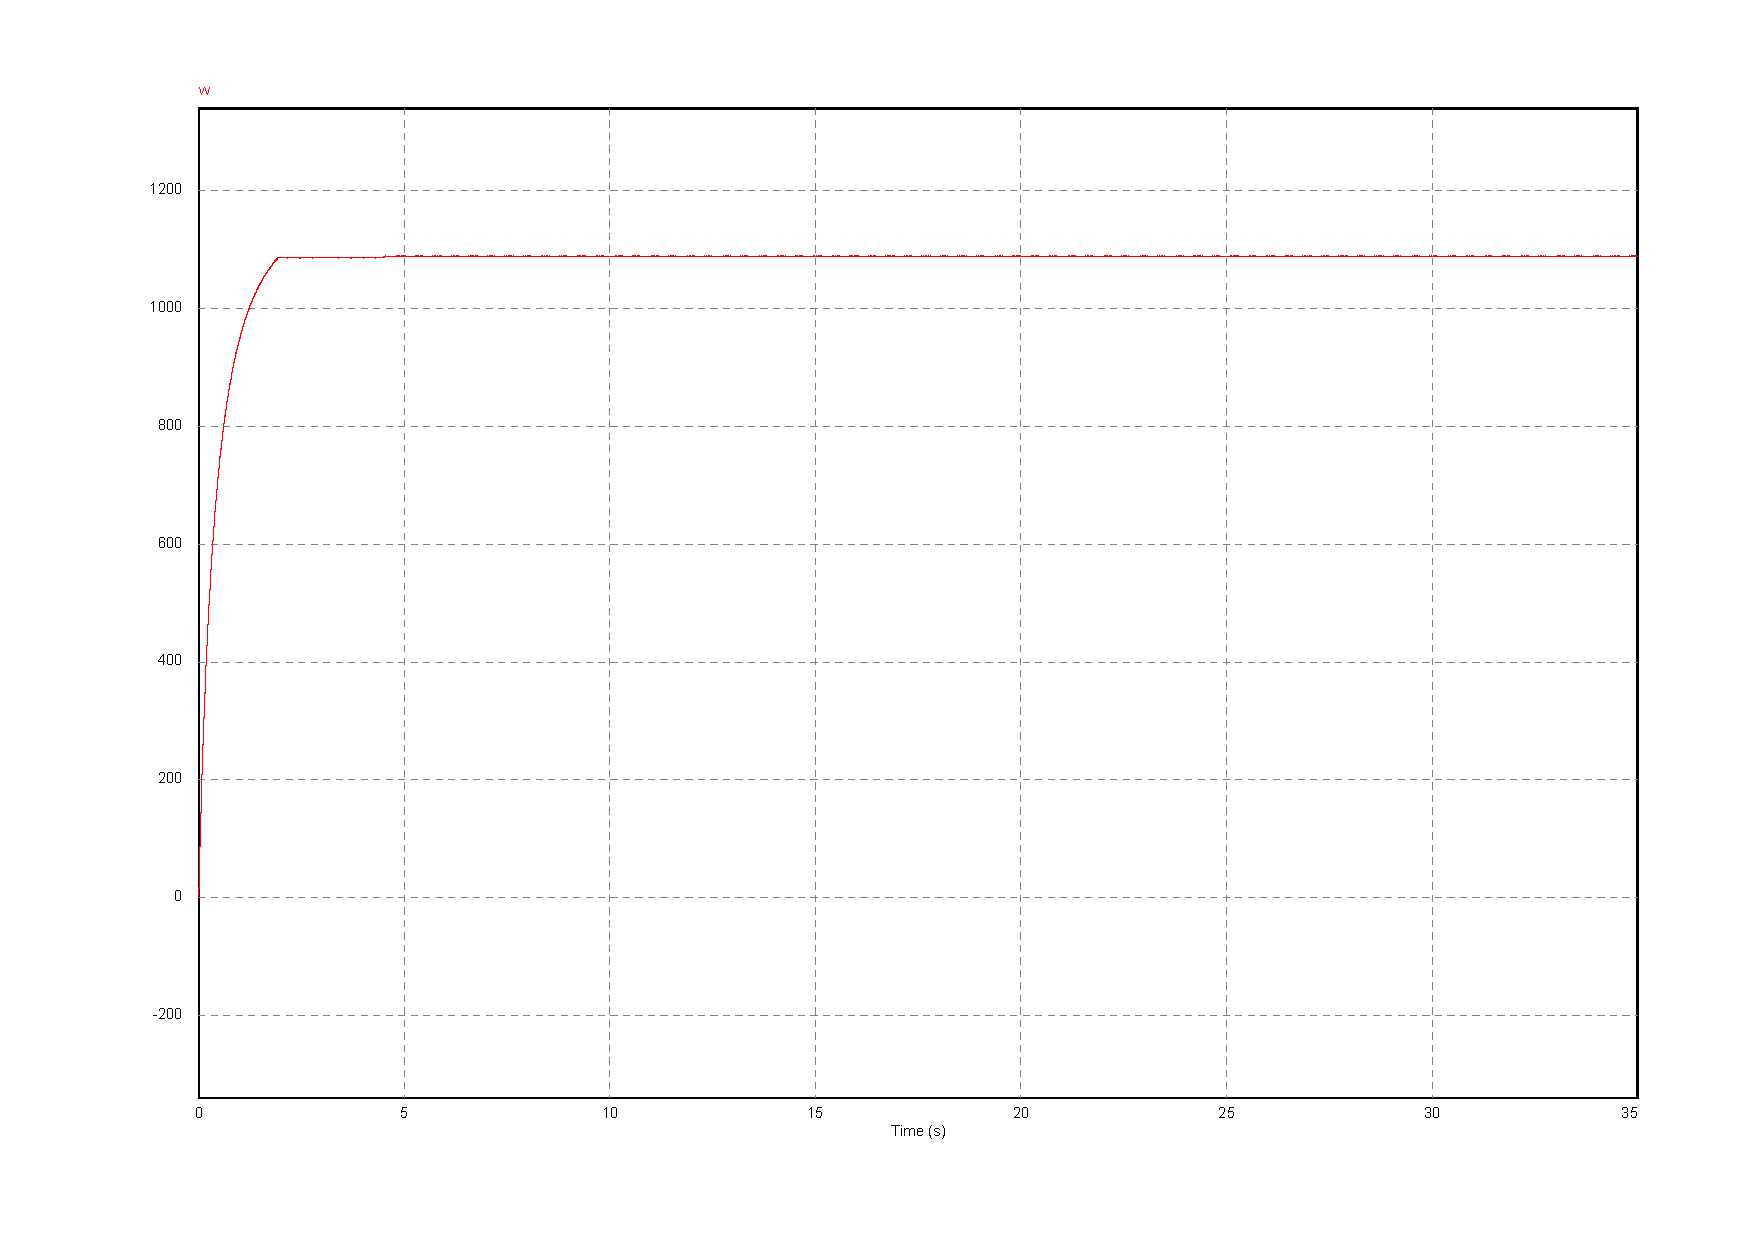
\includegraphics[scale=.33]{images-chude6/chinh-luu-cau-1pha-ban-dieu-khien-bat-doi-xung-tai-motor-DC-plot-w-alpha-30.pdf}}
		\put(80,6){$\alpha = 30^0$}
	\end{picture}
\end{frame}

\begin{frame}{CLưu toàn kỳ bán ĐK}
\begin{picture}(100,100)
%	\vspace{-1.5cm}
		\put(0,-50){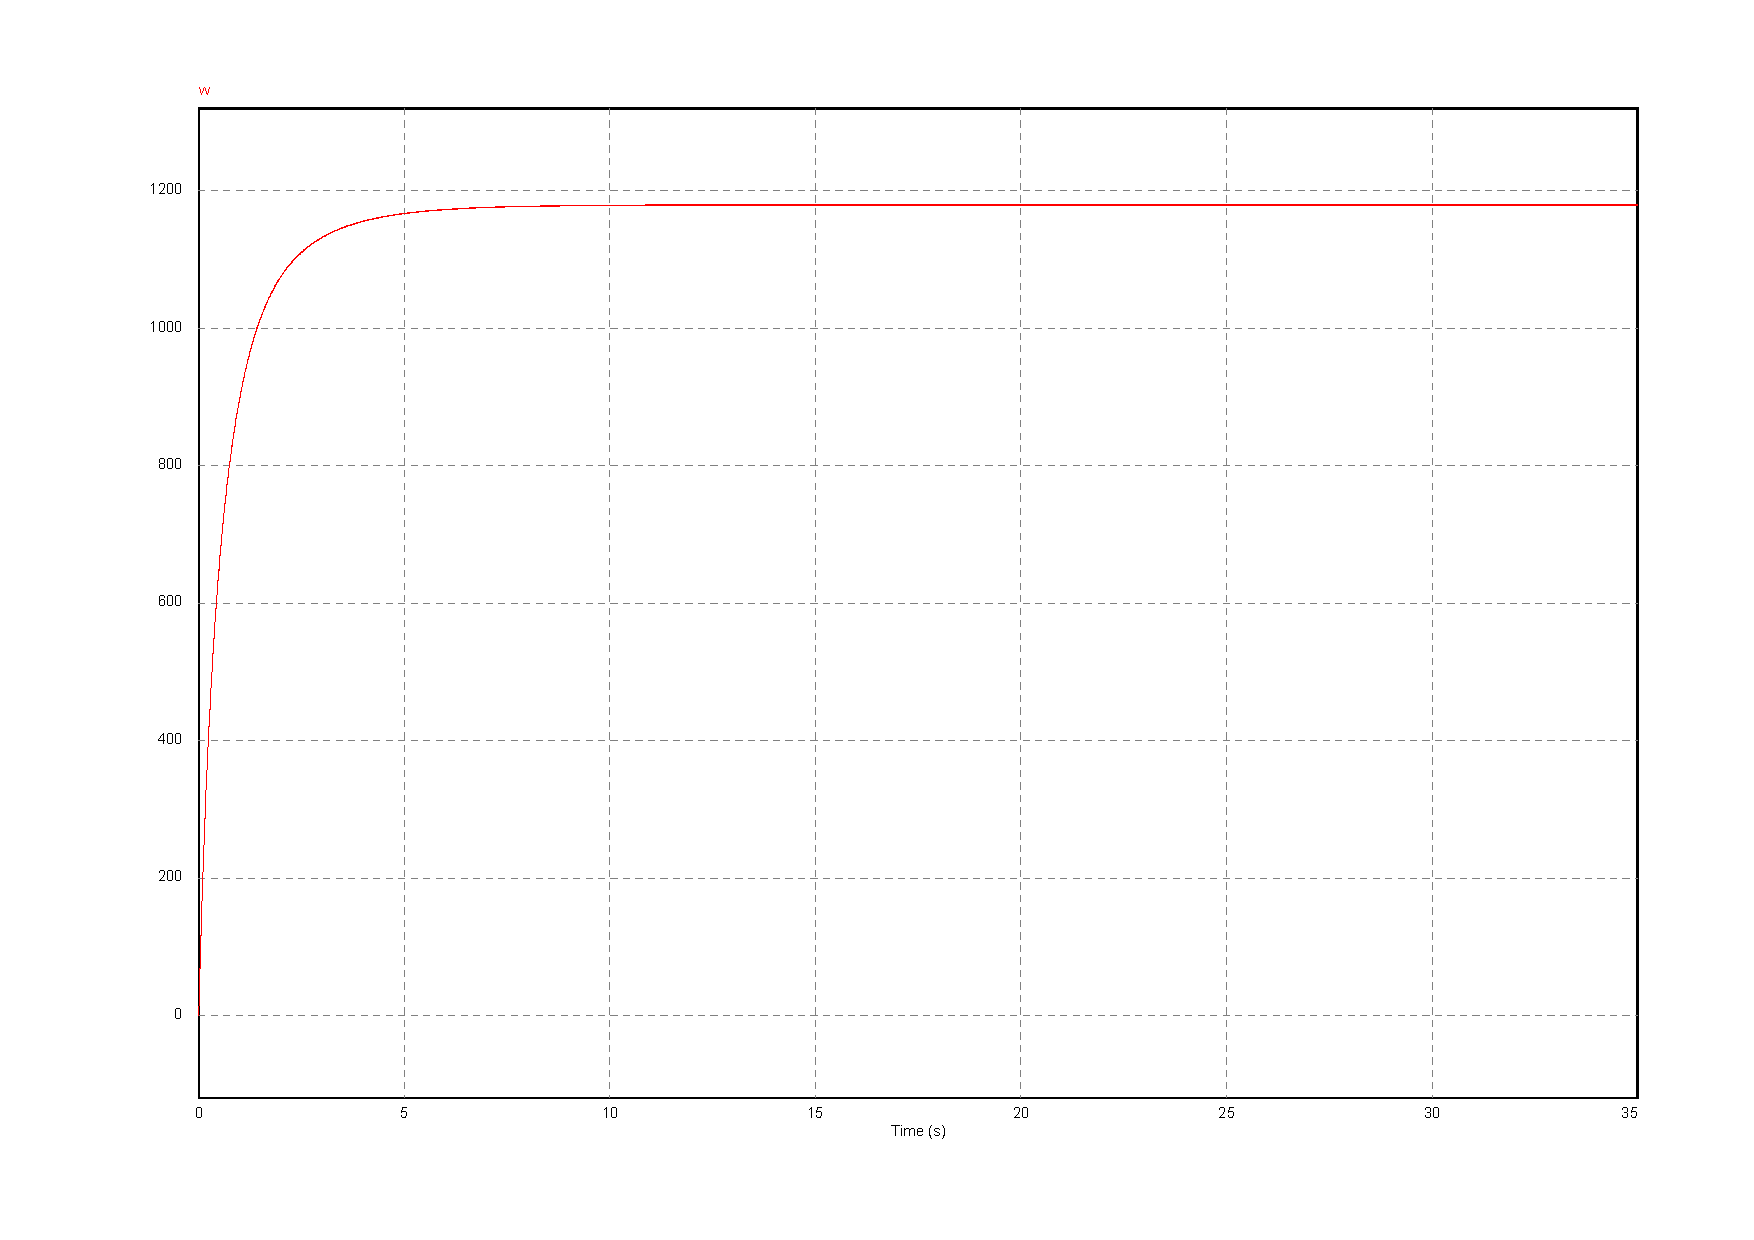
\includegraphics[scale=.33]{images-chude6/chinh-luu-cau-1pha-ban-dieu-khien-bat-doi-xung-tai-motor-DC-plot-w-alpha-60.pdf}}
		\put(80,6){$\alpha = 60^0$}
	\end{picture}
\end{frame}

\begin{frame}{CLưu toàn kỳ bán ĐK}
\begin{picture}(100,100)
%	\vspace{-1.5cm}
		\put(0,-50){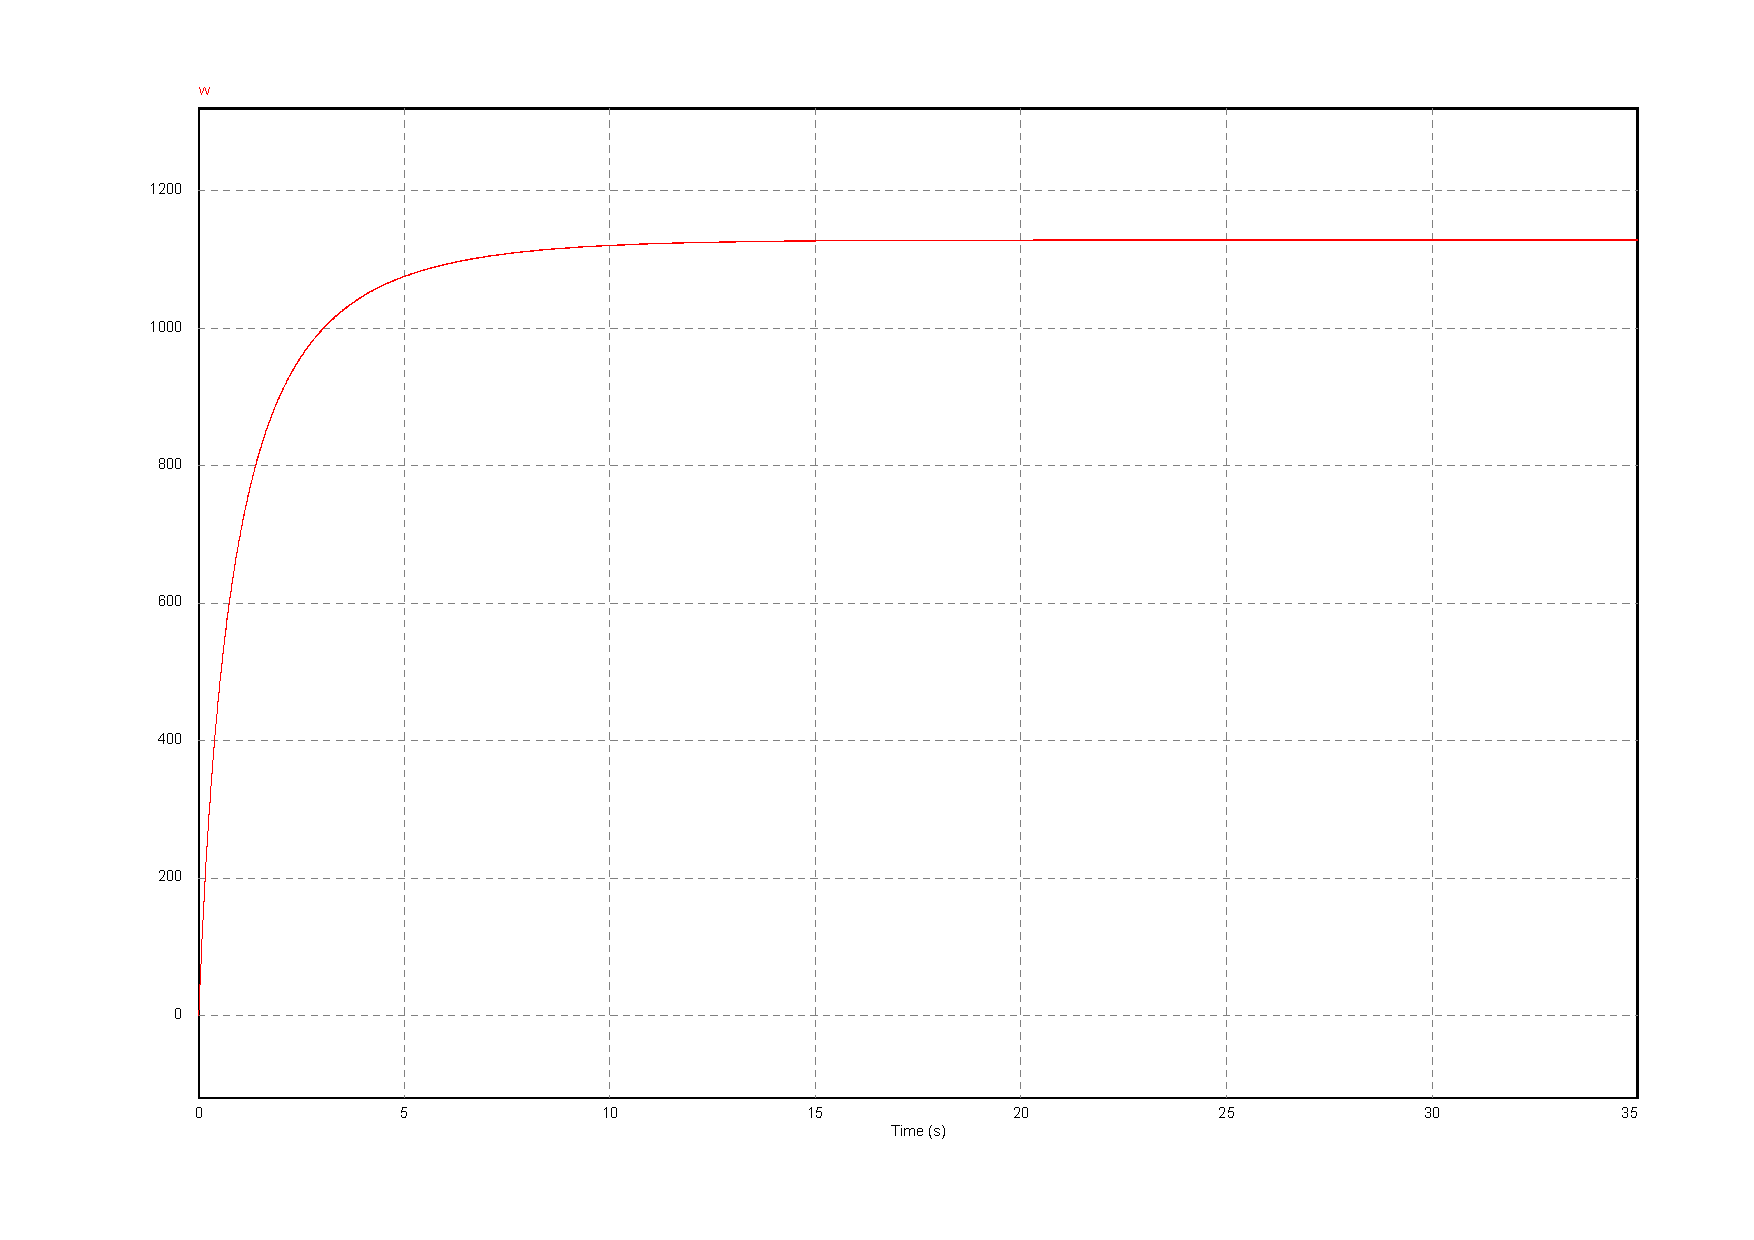
\includegraphics[scale=.33]{images-chude6/chinh-luu-cau-1pha-ban-dieu-khien-bat-doi-xung-tai-motor-DC-plot-w-alpha-90.pdf}}
		\put(80,6){$\alpha = 90^0$}
	\end{picture}
\end{frame}

\begin{frame}{CLưu toàn kỳ bán ĐK}
\begin{picture}(100,100)
%	\vspace{-1.5cm}
		\put(0,-50){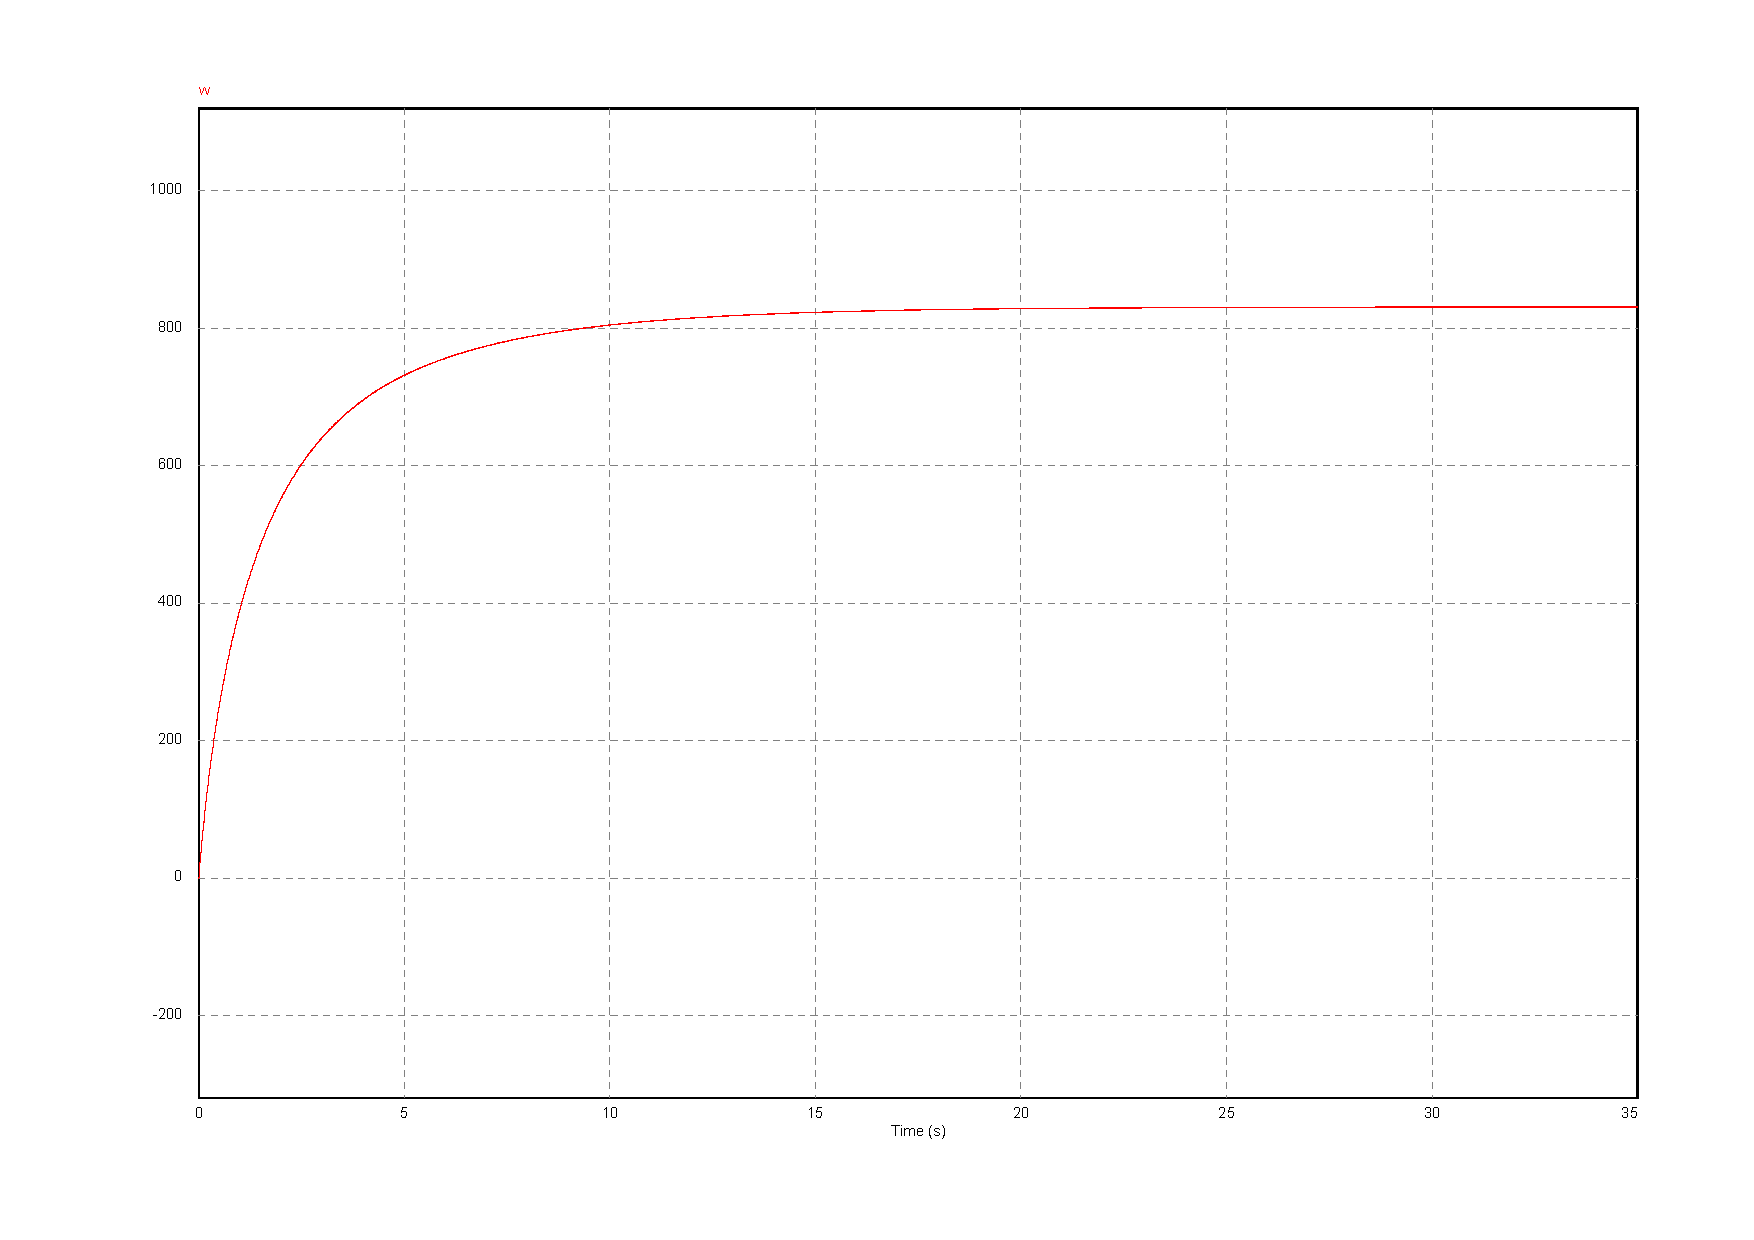
\includegraphics[scale=.33]{images-chude6/chinh-luu-cau-1pha-ban-dieu-khien-bat-doi-xung-tai-motor-DC-plot-w-alpha-120.pdf}}
		\put(80,6){$\alpha = 120^0$}
	\end{picture}
\end{frame}

\begin{frame}{CLưu toàn kỳ bán ĐK}
	\begin{block}{Nhận xét}
	\justifying
		Khi \alert{tăng góc kích $\alpha$} thì \alert{thời gian tăng tốc} của ĐC đến khi đạt tốc độ xác lập cũng \alert{tăng theo} và \alert{tăng nhanh hơn mạch chỉnh lưu 1 tia}.
	\end{block}
\end{frame}

%--------------------------------------------------------------------------------
%--------------------------------------------------------------------------------
% Mạch chỉnh lưu 3 pha
\section[Bộ chỉnh lưu ba pha]{ĐK tốc độ động cơ DC từ bộ chỉnh lưu ba pha}
\begin{frame}{ĐK tốc độ ĐC DC từ bộ chỉnh lưu ba pha}
	\begin{block}{Chỉnh lưu ba pha có điều khiển}
		\begin{itemize}
		\justifying
			\item CLưu cầu bán ĐK.
			\item CLưu cầu ĐK hoàn toàn.
		\end{itemize}
	\end{block}
\end{frame}

\subsection*{Bán điều khiển}
\begin{frame}{CLưu cầu 3P bán ĐK}
	\begin{center}
		\vspace{-.3cm}
		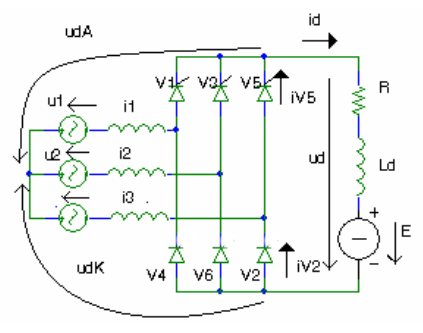
\includegraphics[scale=.55]{images-chude6/chinh-luu-cau-3pha-ban-dieu-khien.png} 
	\end{center}
\end{frame}

\begin{frame}{CLưu cầu 3P bán ĐK}
	\justifying
	$\ast$ Nhận xét:
	
	-- Tốc độ ĐC phụ thuộc vào góc kích $\alpha$.
	
	-- ĐC hoạt động ở góc phần tư thứ nhất.	

	-- Không  hãm được ĐC.
\end{frame}

\subsection*{Điều khiển hòan toàn}
\begin{frame}{CLC 3P ĐK hoàn toàn}
	\begin{center}
		\vspace{-.3cm}
		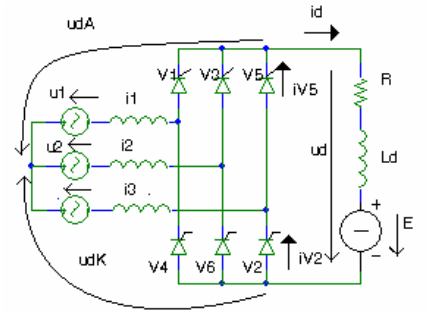
\includegraphics[scale=.55]{images-chude6/chinh-luu-cau-3pha-dieu-khien-hoan-toan.png} 
	\end{center}
\end{frame}

\begin{frame}{CLC 3P ĐK hoàn toàn}
	\justifying
	$\ast$ Nhận xét:
	
	-- Tốc độ ĐC phụ thuộc vào góc kích $\alpha$.
	
	-- ĐC hoạt động ở góc phần tư thứ nhất và thứ tư.		
\end{frame}

%--------------------------------------------------------------------------------
%--------------------------------------------------------------------------------
% Tài liệu tham khảo
\section*{Tài liệu tham khảo}
\begin{frame}{Tài liệu tham khảo}
\begin{small}
\justifying
[1]. Nguyễn Văn Nhờ, \textit{Cơ sở Truyền động điện}, NXB ĐH Quốc gia HCM.

[2]. Nguyễn Văn Nhờ, \textit{Điện tử công suất 1}, NXB ĐH Quốc gia HCM.
\end{small}
\end{frame}
%--------------------------------------------------------------------------------
%--------------------------------------------------------------------------------
% Lời cảm ơn
\section*{Lời cảm ơn}
\begin{frame}
\justifying
\large \alert{Cảm ơn Thầy và các bạn đã quan tâm theo dõi phần trình bày của nhóm!}
\end{frame}
\end{document}